%%%%%%%%%%%%%%%%%%%%%%%%%%%%%%%%%%%%%%%%%%%%%%%%%%%%%%%%%%%%%%%%%%%%%%%%
%                                                                      %
% LaTeX, FIIW thesis template                                          %
%                                                                      %
%%%%%%%%%%%%%%%%%%%%%%%%%%%%%%%%%%%%%%%%%%%%%%%%%%%%%%%%%%%%%%%%%%%%%%%%
\documentclass[11pt,a4paper]{report}
% Indien je je thesis recto-verso wil afdrukken gebruik je onderstaande opties i.p.v. bovenstaande
%\documentclass[11pt,a4paper,twoside,openright]{report}

% user defined packages
\usepackage[ruled,vlined]{algorithm2e}
\usepackage{amsfonts}
% pre-defined packages
\usepackage[a4paper,left=3.5cm, right=2.5cm, top=3.5cm, bottom=3.5cm]{geometry}
\usepackage[english]{babel}
\usepackage{graphicx}
\usepackage[latin1]{inputenc}           % om niet ascii karakters rechtstreeks te kunnen inputten
%\usepackage[utf8]{inputenc}            % commentarieer deze regel uit als je utf8 encoded files gebruikt in plaats van latin1
\usepackage{natbib}
\usepackage{listings}             		 % voor het weergeven van broncode
\usepackage{verbatim}					% weergeven van code, commando's, ...
\usepackage{hyperref}					% maak PDF van de thesis navigeerbaar
\usepackage{url}						% URL's invoegen in tekst met behulp van \url{http://}
\usepackage[small,bf,hang]{caption}     % om de captions wat te verbeteren
\usepackage[final]{pdfpages}            % gebruikt voor het invoegen van het artikel in pdf-formaat
\usepackage{pslatex}					% andere lettertype's dan de standaard types
\usepackage{lipsum}
\usepackage{sectsty}					% aanpassen van de fonts van sections en chapters
%\usepackage[nottoc,numbib]{tocbibind}	% Bibliography mee in de ToC

\allsectionsfont{\sffamily}
\chapterfont{\raggedleft\sffamily}

\usepackage{float}                      % De optie H voor de plaatsing van figuren op de plaats waar je ze invoegt. bvb. \begin{figure}[H]
%\usepackage{longtable}					% tabellen die over meerdere pagina's gespreid worden
\usepackage[times]{quotchap}           % indien je fancy hoofdstuktitels wil
%\usepackage[none]{hyphenat}
%\usepackage{latexsym}
\usepackage{amsmath}
\usepackage{mathtools}
%\usepackage{amssymb}

% MFA: zet zoekpad voor figure
\graphicspath{{fig/}}

\usepackage{fiiw}
% \usepackage{fiiw_eng} % For the english version (also change last page at the bottom of this file!

%door onderstaande regels in commentaar te zetten, of op false, kan je pagina's weglaten
%bijvoorbeeld het weglaten van een voorwoord, lijst met symbolen, ...
%%%%%%%%%%%%%%%%%%%%%%%%%%%%%%%%%%%%%%%%%%%%%%%%%%%%%%%%%%%%%%%%%%%%%%%%%%%%%%%%%%%%%%%%
%voorwoord toevoegen?
\acknowledgementspagetrue
\acknowledgements{voorwoord}			%.tex file met daarin het voorwoord

%samenvatting toevoegen
\summarypagetrue
\summary{samenvatting}					%.tex met daarin de samenvatting

%abstract toevoegen?
\abstractpagetrue
\abstracts{abstract}					%.tex file met daarin het abstract
%lijst van figuren toevoegen?
\listoffigurespagetrue
%lijst van tabellen toevoegen?
\listoftablespagetrue
%lijst van symbolen toevoegen?
\listofsymbolspagetrue
\listofsymbols{symbolen}				%.tex file met daarin de lijst van symbolen
%lijst van afkortingen toevoegen?
\listofabbrevspagetrue
\listofabbrevs{afkortingen}				%.tex file met daarin de lijst van symbolen

%informatie over het eindwerk, de promotor, ...
%%%%%%%%%%%%%%%%%%%%%%%%%%%%%%%%%%%%%%%%%%%%%%%
\opleiding{Industriele Wetenschappen}
\afdeling{Electronica-ICT}

\campus{denayereng} %denayer,denayereng,geel,geeleng,gent,ghenteng,groept,groupteng,brugge,brugeseng

% onder embargo? laat leeg indien van niet; vul de datum in als dd-mm-yyyy indien van wel
\embargo{}

\title{Secure face matching}
\subtitle{}
% \author{naam student}
\forenameA{Felix}
\surnameA{Lerner}

% l
\forenameB{}
\surnameB{}

\academicyear{2019 - 2020}

\promotorA[Promotor]{Prof. dr. ir. Toon Goedem{\'e}}
%\promotorB[Co-promotor(en)]{Prof. dr. ir. Andere Baas}
\promotorC[Co-promotor:]{Dr. Pradip Mainali (Onespan)}

\begin{document}
%\selectlanguage{dutch}
\selectlanguage{english} % For the english version
\preface

%%%%%%%%%%%%%%%%%%%%%%%%%%%%%%%%%%%%%%%%%%%%%%%%%%%%%%%%%%%%%%%%%%%
%                                                                 %
%                            CHAPTER                              %
%                                                                 %
%%%%%%%%%%%%%%%%%%%%%%%%%%%%%%%%%%%%%%%%%%%%%%%%%%%%%%%%%%%%%%%%%%%

\chapter{Introduction}
Deep learning-based object detection on images is a hot topic for researchers and interest in machine learning is steadily growing among miscellaneous businesses. Facial recognition is one of the many applications machine learning has to offer. A face recognition algorithm tries to recognise faces of the same person. Faces are very unique parts of our body, thus face matching can be used as a means to do biometric authentication. In this case, a client sends a picture containing their face to an external service which grants the client access if the face is similar to the one stored in the database.

More and more users are concerned about their privacy and the security of their data stored and processed on servers. Not only are they afraid of malicious hackers stealing their sensitive data, they also fear the servers operator will use their data for purposes other than the user agreed to. Big corporations have been found guilty of collecting user data for unethical purposes (source: \cite{cadwalladr2018revealed}).

Secure multiparty computation (MPC) is a subfield of cryptography, making it possible for a party to run an algortihm on confidential data, that is supposed to stay unknown even to the party running the algorithm. There exist different methods to perform privacy-preserving computations, MPC is the one we will use.

Secure Multiparty Computation and Machine Learning aren't new concepts, in fact they exist for over 40 years. But with the rise of big data and processing power lately, there has been an increase in research into these fields.

Because of these concerns researchers are looking for technologies to enhance the privacy of the user during the processing of it's data on a server.

Onespan\footnote{Onespan's official website: \url{https://www.onespan.com}} (formerly VASCO Data Security International, Inc.) is a global company were most of our research was done. Onespan offers a series of security and authentication products and technologies and specializes in digital identity and anti-fraud solutions. The company continues to be active in research and innovation in different fields of technology, especially cryptography and data science.

In this thesis we study the applicability of MPC protocols on deep learning-based face matching algorithms and try to implement a privacy-preserving face matching algorithm.

\section{Problem}
The use of third party MLaaS (Machine Learning as a Service) providers or any cloud computing solution, as processing power for an image classification task, raises privacy concerns as sensitive images of users need to be sent to servers running an instance of the neural network.

It's important to note that the transport of the image from the client to the server is deemed to be secure, since the parties can make use of reliable HTTPS (Hypertext Transfer Protocol Secure) connections.

The user's images, however, are stored in plaintext \footnote{plaintext or cleartext are common cryptographic terms for unencrypted data.} on the server, as well as the computed output of the image.

Furthermore the whole design of the neural network including all trained parameters needs to be stored on the servers of the third party, for the image classifier to function. Both of these remote processing solutions require a considerably amount of trust in the third party. Since the third party could potentially exploit the user data for commercial purposes or even steal the intellectual property of the image classifier. Of course most cloud computing service providers are not inherently malicious. But as long as the user's data is stored in cleartext on the server, there is a risk that the service provider could turn malicious. Or even worse, hackers could break in to the server and breach the confidential user data.

In this thesis we try to tackle the need to trust a third party MLaaS provider. We want it to compute an encrypted image on an obfuscated neural network to ouput a correct encrypted result. This encrypted result shall be sent to the client, which will then decrypt it. Figure \ref{fig:intro_overview} shows an oversimplified overview of this algorithm.

\begin{figure}[H]
  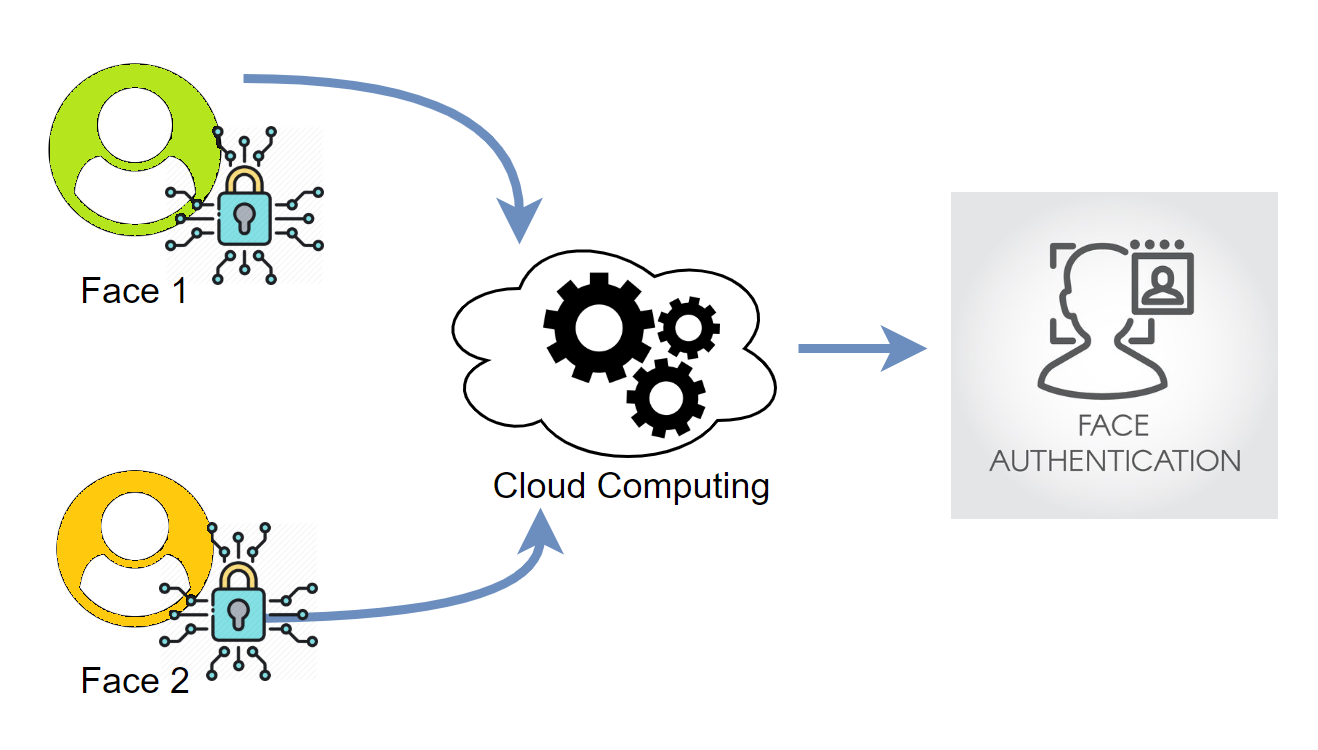
\includegraphics[scale=0.4]{fig/intro_overview.png}
  \centering
  \caption{Overview of secure face matching. The cloud computing services compute over encrypted inputs.}
  \label{fig:intro_overview}
\end{figure}

Before we begin specifying our hypotheses, lets define some frequently occuring terms:

\begin{itemize}
  \item Encryption: the process of converting data into a code, to ensure confidentiality and prevent unauthorized access.
  \item Privacy-preserving/secure algorithms: Algorithms that allow computation of private data, while preserving privacy.
  \item Face matching algorithm: Set of rules that a computer uses to compare two faces, to determine wheter there is a match.
\end{itemize}

\section{Hypothesis}
\label{chapter:hypothesis}
\paragraph{How can we securely compute the inference of a deep learning-based facial recognition neural network?}\mbox{} \\
With the use of MPC protocols we can implement methods such that we can compute a whole face recognition convolutional neural network on an encrypted image of a face. This preserves the privacy of the user while allowing the computation to be outsourced to an untrusted third party.
\paragraph{How can we optimize the secure facial recognition task to run more efficiently?}\mbox{}
\\
We predict a drastic decrease in perfomance when running inference on the privacy-preserving neural network, because MPC is a protocol over a network of parties the computational time will not be the only factor to account for. We will try to find performance optimizations along the way of implementing a proof of concept by looking at existing optimization concepts for MPC as well as optimization solutions for neural networks.

%%%%%%%%%%%%%%%%%%%%%%%%%%%%%%%%%%%%%%%%%%%%%%%%%%%%%%%%%%%%%%%%%%%
%                                                                 %
%                            CHAPTER                              %
%                                                                 %
%%%%%%%%%%%%%%%%%%%%%%%%%%%%%%%%%%%%%%%%%%%%%%%%%%%%%%%%%%%%%%%%%%%

\chapter{Literature study}

\section{Convolutional neural network}
Convolution neural networks (CNN) is a special type of neural network used for images. The spatial properties of the pixels in the image are used during the evaluation of the input, meaning the neighbouring pixels of a central pixel impact the output to the next layer of that central pixel while pixels further away do not.
CNNs are made of multiple layers. Typically, as you move further from the input layer to the output layer the dimensionality reduces, we can say the input gets mapped on a desired output manifold. Inputs that we classify as similar are supposed to be in the same region in the output manifold.

\subsection{Convolution layer}
In this layer a discrete convolution of a kernel $K$ shifting over an image $I$ is performed, as shown in equation \ref{eq:1}. The kernel has parameters also called weights, so that certain features get extracted from the input.
\begin{equation} \label{eq:1}
  (I*K)[m,n]=\sum_j\sum_k I[m-j,n-k]K[j,k]
\end{equation}
The output of this layer is a convolved feature map.

\subsection{Activation function}
Since these convolutions are simple lineair operations and most image classification tasks require non-lineair classifiers, non-lineairity needs to be added to the neural network. This is achieved through adding a non-linear activation function after a convolution or fully connected layer. The most popular activation function is the rectified linear unit (ReLU) as seen in equation \ref{eq:2}.
\begin{equation} \label{eq:2}
  f(x)=max(0,1)
\end{equation}

\subsection{Pooling layer}
The dimensionality reduction we talked about in the beginning of this chapter happens in the pooling layer. A kernel is shifted over the image. In the case of max pooling the kernel selects the maximum value of the portion of the image it covers, to create the new dimensionality reduced image.

\subsection{Fully connected layer}
The fully connected layer is a multilayer perceptron that discriminates different object classes and identifies identical ones. All elements in vector $h_{i-1}^{out}$ have their own bias $B_i$ and weight $W_i$ so that $h_i^{in}$ can be calculated for each layer $i$ according to equation \ref{eq:3}.
\begin{equation} \label{eq:3}
  h_i^{in} = h_{i-1}^{out} \cdot W_i + B_i
\end{equation}

\section{Secure multiparty computation}
Secure multiparty coputation is a protocol that is used between $n$ number of parties $P$. Each of these parties has private data also called a secret $S$. With MPC it is possible for these parties to compute a public\footnote{public or global means known to all parties, while private or local means known only by the corresponding party} function $f$ on the secrets. Such that a party $p_i \in P$ only knows his secret $s_i \in S$ and the public securely computed output $f(s_0,s_2,s_{n-1})$ after the protocol has succesfully finished.
\newline
A classic application is Yao's Millionaires' problem \cite{yao1982protocols} in wich two millionaires wish to know who is richer, there is catch however. Instead of making their balances publicly known. They wish to keep their balances a secret. In this case the number of parties $n$ is 2 the secrets $s_0$ and $s_1$ are their balances. The public function $f(s_0,s_1)=1$ if $s_0<s_1$ and $0$ otherwise.

We categorize 2 types of parties based on their willingness to deviate from the correct predefined protocol.
\begin{itemize}
  \item Honest but curious parties (passive): Parties wish to know other parties secrets but will not deviate from the protocol at any time.
  \item Malicious parties (active): Parties wish to know other parties secrets and wish to change output of computation to favourable result. Parties will deviate from the protocol to cheat and change the outcome at any time.
\end{itemize}

If the two millionaires are honest but curious parties, they will not deviate from the protocol and they will computer the correct output as a result they will know who is the richer millionair but they won't know how much money the other one has. In the other case one of the two millionaires is corrupt and acts maliciously, the honest millionair will follow protocol while the dishonest millionair will deviate from the protocol to change the result in his favour. In the event that the dishonest millionair is poorer he will change the outcome thus appearing richer.
From now on, we assume the parties are honest but curious parties, unless specified otherwise. We also assume the communication between the different parties to be secure.

\subsection{Secret sharing}
In order to do secure computing, the parties need to split their secret into secret shares. A secret sharing method can be used by the secret holder to split a secret into a number of shares. Combining these shares will reveal the secret, while individual shares alone will leak nothing about the secret. In a $(t,n)$ threshold secret sharing sheme parties must combine atleast $t$ shares of the total $n$ shares, to obtain the secret. We can now set a threshold $t$ high enough, denying the secret to small curious parties and allowing to reveal the secret when a majority ($\geq t$) consensus is reached. Shamir's secret sharing scheme \cite{shamir1979share} is based on polynomial interpolation and the essential idea is that it takes atleast $t$ points in order to define a polynomial $p(x)$ of degree $t-1$. Given a set of $t$ points in a 2-dimensional carthesian system  $(x_1, y_1), (x_2, y_2), ..., (x_t,y_t)$, there exists only one polynomial of degree $t-1$. This can be proven and the mathematical construction of a polynomial $p(x)$ of degree $t-1$ based on a set of $t$ points can be calculated using Lagrange's interpolation formula \ref{eq:5}.

\begin{equation} \label{eq:5}
\begin{aligned}
  p(x)= \sum_{i=1}^{t}y_{i}\delta_{i}(x)\text{\space\space\space\space with\space\space }\delta_{i}(x)=\prod_{1\leq j<t; i\neq j} \frac{x-x_i}{x_j-x_i}
\end{aligned}
\end{equation}

With this in mind, a secret dealer can now share his secret $s$ to $n$ parties by choosing a random $t-1$ degree polynomial $p(x)=a_{0} + a_{1}x + ... + a_{t-1}x^{t-1}$ in which $a_{0}$ is the secret or the number representation of the secret if the secret is not a number. The dealer now calculates $n$ points on the polynomial starting from $x=1$, because the secret is located at $x=0$. Each party $p_i \in {p_1, p_2, ..., p_n}$ is given a different single point $(x_i,y_i)$, at this stage the secret is shared. To recombine the secret, the parties simply broadcast or send their shares to a central entity, if more than $t$ shares are known, it suffices to calculate the Lagrange polynomial $p(x)$ and $s=p(0)$. In the case of not having enough shares, the Lagrange polynomial becomes impossible to calculate since every polynomial is equally likely, thus revealing absolutely nothing about the secret.

\subsection{Operations}
\subsubsection{Artithmetic operators}
\subsubsection{Relational operators}
\subsection{Share recombination}

\section{Conclusion}

%%%%%%%%%%%%%%%%%%%%%%%%%%%%%%%%%%%%%%%%%%%%%%%%%%%%%%%%%%%%%%%%%%%
%                                                                 %
%                            CHAPTER                              %
%                                                                 %
%%%%%%%%%%%%%%%%%%%%%%%%%%%%%%%%%%%%%%%%%%%%%%%%%%%%%%%%%%%%%%%%%%%

\NewDocumentCommand{\codeword}{v}{%
\texttt{\textcolor{blue}{#1}}%
}

\DeclarePairedDelimiter\floor{\lfloor}{\rfloor}

\chapter{Implementation}
In this chapter we will explain how we implemented MPC for face matching algorithms. We will do this by giving a high-level overview of the system and then diving deeper in more interesting parts. We also show some techniques to lose some complexity without losing too much accuracy. With the information in this chapter and the code in the appendix, you should be able to reproduce our experiments. Feel free to checkout our code by cloning our GitHub repository\footnote{\url{https://github.com/Fluxmux/securefacematching}}.

\section{Specifications}
There are two major subprojects. The first subproject (chapter \ref{Deep Learning}) is making sure we can generate the appropriate parameters for the face matching network. It is important that the model is accurate enough. The second subproject (chapter \ref{Secure Functions}) is about transforming the classic machine learning functions to secure ones. To add this security or privacy-preserving factor we use a MPC framework.

\subsection{Deep Learning}
\label{Deep Learning}
A machine learning project usually includes on of the popular frameworks available to the public. Since we were already familiar with Pytorch we used this library as a python package.

Pytorch \footnote{\url{https://pytorch.org}} provides us with a deep learning research platform that provides maximum flexibility and speed. It's fairly easy to use but that doesn't mean we can't design more complex models or features. Pytorch uses tensors, tensors are multi-dimensional matrix containing elements of a single data type. Designing a neural network with Pytorch is as simple as defining a class with the layers in the correct order. An example of a neural network written using pytorch can be seen in the following code (listing~\ref{lst:pytorch_example})\\

\begin{lstlisting}[language=Python, caption={Pytorch neural network example}, label={lst:pytorch_example}, frame=single]
class SiameseNetwork(nn.Module):
    def __init__(self):
        super(SiameseNetwork, self).__init__()

        self.cnn = nn.Sequential(
            nn.ReflectionPad2d(1),
            nn.Conv2d(1, 16, kernel_size=5),
            nn.ReLU(inplace=True),
            nn.BatchNorm2d(16),
            nn.MaxPool2d(kernel_size=2, stride=2),
            ...
        )
\end{lstlisting}

Making an accurate face matching neural network. Is a process that involves three major steps.

First of all the design or architecture of the network gets chosen. There exist a number of different topologies used in deep neural networks. But often choosing which one to take and how many layers to use, is the most difficult task. We will cover the architecture of the model in chapter \ref{ConvolutionalNeuralNetworkArchitecture}. Adding more layers is the same as adding more parameters. And a model with more parameters is more complex.

The second step is called the traing of the neural network. Training is done using a part of the dataset that is specific for training and shouldn't be used for anything else.

A typical workflow of the training step looks something like this: Two labeled faces are sent seperatly sent through the network. The euclidean distance (equation \ref{eq:euclideandistance}) for inputs $\vec{X_{1}}$ and $\vec{X_{2}}$ and the parameterized function $G_{W}$ calculates the distance between the outputs. This distance metric should be close to zero for faces belonging to the same person. But as large as possible for faces belonging to different person.

\begin{equation} \label{eq:euclideandistance}
  D_{W}(\vec{X_{1}},\vec{X_{2}})=\lVert G_{W}(\vec{X_{1}}) - G_{W}(\vec{X_{2}}) \rVert
\end{equation}

Then we use the loss function Yann LeCun first introduced in his paper \cite{hadsell2006dimensionality}; The general loss function $L$ is the sum of contrastive loss functions for a training pair in the set of training pairs of size $P$.

Let $Y$ be the binary label assigned to this pair of faces, $Y=0$ if $\vec{X_{1}}$ and $\vec{X_{2}}$ are labeled as similar, and $Y=1$ if $\vec{X_{1}}$ and $\vec{X_{2}}$ are labeled as dissimilar.

\begin{equation} \label{eq:contrastiveloss}
  L(W,Y,\vec{X_{1}},\vec{X_{2}})=(1-Y)\frac{1}{2}(D_{W})^{2} + Y\frac{1}{2}(max^{2}(0, m - D_{W}))
\end{equation}

The contrastive loss function is definded in formula \ref{eq:contrastiveloss}, where $m > 0$ is the margin. The margin $m$ can be seen as a radius so that dissimilar pairs still contribute to the loss function if their distance is withing this radius. The goal of training is to minimize the loss. For similar pairs this means decreasing the distance $D_{W}$, for dissimilar pairs this means increasing the distance to be greater than the margin. We came to the conclusion that our loss reduces the most if we choose a margin of $m=2$.

We also tried a different approach, instead of using this distance metric (which we would than have to statically threshold) we would like to have a probability value between $0$ and $1$. The output layer of the network consists out of two neurons (two classes), one neuron describes the similar faces, the other neuron describes the dissimilar faces. A probability of $0$ means that the faces belong to different persons and a probability of $1$ means that the faces belong to the same person. Binary Cross Entropy loss, or Logaritmic loss (equation \ref{eq:crossentropyloss}) is one of the loss functions that can be used to achieve this.

\begin{equation} \label{eq:crossentropyloss}
  L=-{(y\log(p) + (1 - y)\log(1 - p))}
\end{equation}

Let $y$ be the binary label assigned to this pair of faces, $p$ is the predicted probability. To visualize this loss function, have a look at figure \ref{fig:crossentropyloss}

\begin{figure}[H]
  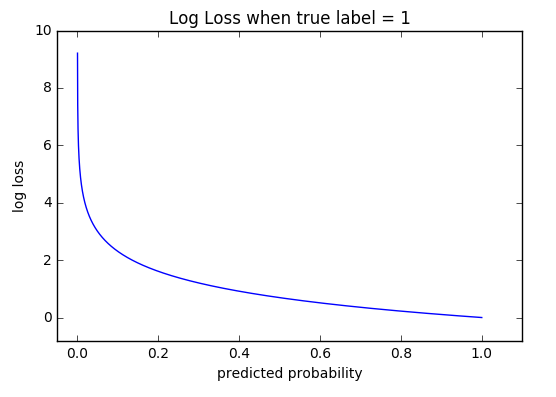
\includegraphics[scale=0.6]{fig/cross_entropy.png}
  \centering
  \caption{Range of loss values for $y=1$}
  \label{fig:crossentropyloss}
\end{figure}

There exist a great number of other functions. Some might be better suited for the face matching problem. But since we need to keep things simple in order to implement MPC. We opt for one of the two loss functions described above.

Training a neural network takes some time, but the process can be sped up by using graphics processing units (GPU). We were lucky enough to have a dedicated GPU server at our disposal. While training the network is an easy task, we should look out for overfitting or underfitting.

Overfitting a model happens when there are too much parameters for a model or when the training was performed for too long. It will perform poorly on the validation dataset (part of dataset used to detect bad trainig behaviour) while performing excellent on the training dataset. There are two ways of overcoming overfitting. One way is to make the training dataset larger. Having more samples to train on, generalizes the learning model better. The other way is to design the model with fewer parameters, making it less complex. We use learning curves to track the training process of our face matching algortihm. An example of a more or less correct learning curve can be found in figure \ref{fig:trainingcurve}.

\begin{figure}[H]
  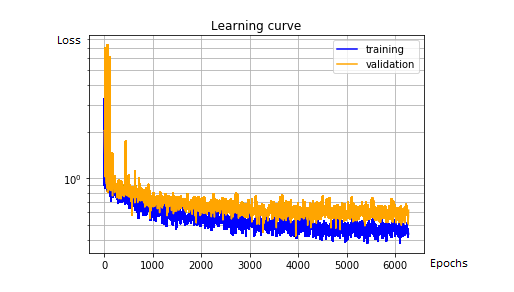
\includegraphics{fig/trainingcurve.png}
  \caption{Learning curves are used to track the training of a model}
  \label{fig:trainingcurve}
\end{figure}

Underfitting happens when a machine learning algorithm cannot capture the underlying structure of data. The model can't fit the data enough. Underfitting is more difficult to spot but easier to overcome. We can overcome this problem by making our model more complex.

As you can see by now, the architecture of a model is extremely important for it to function as wished.

The third step also called the hyperparameter tuning or hyperparameter optimization step, is what makes a good machine learning model even better. This process is not at all logic, experience and intuition can facilitate this. Hyperparameters are all the parameters whose values are set before the learning process begins. There are different methods for optimizing hyperparameters, since we wanted to learn the model and how it behaves relating to small changes in the values of the hyperparameters we went for Manual Random Search. Note that this took us some time because this involves multiple training steps. But since we had a GPU server at our disposal we could parallelize this task. In our case this step improved our accuracy by about 5\%.

We used the Database of Faces\footnote{\url{http://cam-orl.co.uk/facedatabase.html}} to train and test our face matching algortihm. The dataset contains a set of 10 images of frontal faces with different expressions per person and a total of 40 persons. The pictures are in pgm format which is extremely easy to interact with. They have a dimension of 1 x 92 x 112. An example of a set of images from the dataset can be seen in figure \ref{fig:databaseoffaces}. We divided the dataset in to 3 parts: 75\% training, 12.5\% testing and another 12.5\% for validation.

\begin{figure}[H]
  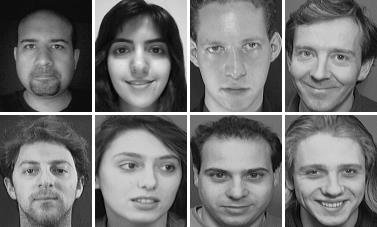
\includegraphics[scale=0.7]{fig/databaseoffacess.png}
  \centering
  \caption{Example of faces in dataset}
  \label{fig:databaseoffaces}
\end{figure}

\subsection{Secure Functions}
\label{Secure Functions}
Secure functions or the privacy preserving equivalent of an ordinary function can be used to compute an encrypted output as a function of encrypted inputs (figure \ref{fig:blackbox}). The protocol used for defining these secure functions is the MPC protocol.

\begin{figure}[H]
  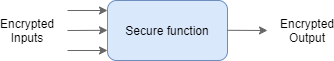
\includegraphics[scale=0.8]{plots/blackbox.png}
  \centering
  \caption{Secure function as a black box}
  \label{fig:blackbox}
\end{figure}

Berry Schoenmakers is a cryptographer working on cryptographic protocols for electronic voting, electronic payments and secure multiparty computation. Since 2018 he has been working on a general MPC implementation for python, called MPyC. This pyhton package can be easily installed with pip: \codeword{pip install mpyc}. The mpyc package defines two new number representation types: SecFxp and SecInt. SecFxp are secure fixed-point numbers. SecInt are secure integers. For more information on how to use this package have a look at the source code at \url{https://github.com/lschoe/mpyc}.

There are number of basic functions predefined, like \codeword{add}, \codeword{sub}, \codeword{mul} and \codeword{div}, respectively $+$, $-$, $\times$ and $\div$. As well as \codeword{eq} (equal to), \codeword{ge} (greater than or equal), \codeword{min} and \codeword{max}. The total set of available functions can be found in \codeword{mpyc.runtime.py}. But for our task the functions noted above are all we need.

With this set of fundamental functions we can generate our own custom functions that serve our needs.

\subsubsection{Custom Operations}

We introduce three essential custom secure functions that can be found in \codeword{custom_operations.py}.

\begin{itemize}
  \item \codeword{convolution}
  \item \codeword{maxpool}
  \item \codeword{relu}
\end{itemize}

\codeword{convolution} is a secure function that takes two arguments $X$ and $W$ as input as can be seen in listing~\ref{lst:convolution}. Let $W$ be the kernel and $X$ the image over which to do the convolution. $X$ can be of any shape $(m, n)$, $W$ needs to be a square matrix of size $s$. We then define $Y$ to be the output matrix of the convolution function. Because the convolution is padded, $Y$ is of the same size as $X$.

\begin{lstlisting}[language=Python, caption={Secure convolution function}, label={lst:convolution}, frame=single, breaklines=true]
def convolution(X, W):
    m, n = dim(X)
    s = len(W)
    s2 = (s - 1) // 2
    Y = [None] * m
    for i in range(m):
        Y[i] = [None] * n
        for j in range(n):
            t = 0
            ix = i - s2
            for di in range(s):
                if 0 <= ix < m:
                    jx = j - s2
                    for dj in range(s):
                        if 0 <= jx < n:
                            t += X[ix][jx] * W[di][dj]
                        jx += 1
                ix += 1
            Y[i][j] = t
    return Y
\end{lstlisting}

Note that the number representation types that will be used in this secure convolution function, are not simple integers or floats. $X$, $W$ and $Y$ are matrices of SecInt's or SecFxp's.\\

\codeword{maxpool} is a secure function (listing~\ref{lst:maxpooling}). The function takes one argument as input, $X$ an image of size $(m,n)$. We define a specific type of max pooling, the pooling window has a size of $2$ by $2$ and the stride is equal to $2$. The output $Y$ is a matrix of size $(\floor*{\frac{m}{2}}, \floor*{\frac{n}{2}})$.

\begin{lstlisting}[language=Python, caption={Secure max pooling function}, label={lst:maxpooling}, frame=single, breaklines=true]
def maxpool(X):
    m, n = dim(X)
    Y = [None] * (m // 2)
    for i in range(0, m - 1, 2):
        Y[int(i/2)] = [None] * (n // 2)
        for j in range(0, n - 1, 2):
            Y[int(i/2)][int(j/2)] = mpc.max(X[i][j], X[i][j+1], X[i+1][j], X[i+1][j+1])
    return np.array(Y)
\end{lstlisting}

\codeword{relu} is a secure function (listing~\ref{lst:relu}). The function takes one argument as input, $X$ the image of size $(m,n)$. This function doesn't change the shape of the input matrix, only the value of the elements of the matrix are changed, if they fulfill the condition.

\begin{lstlisting}[language=Python, caption={Secure ReLU function}, label={lst:relu}, frame=single, breaklines=true]
def relu(X):
    return np.vectorize(lambda a: (a >= 0) * a)(X)
\end{lstlisting}

Note that writing \codeword{a >= 0} or \codeword{mpc.ge(a, 0)} has the same effect. The same can be said for \codeword{(a >= 0) * a} and \codeword{mpc.mul(a >=0, a)}. The MPC operators are wrapped for the basic python operators on SecInt's and SecFxp's.\\

These three basic building blocks are essential for a convolutional neural network. But for the MPC protocol to function properly, we need to address some other problems. We will continue by giving a practical overview of the whole MPC protocol.\\

\begin{figure}[H]
  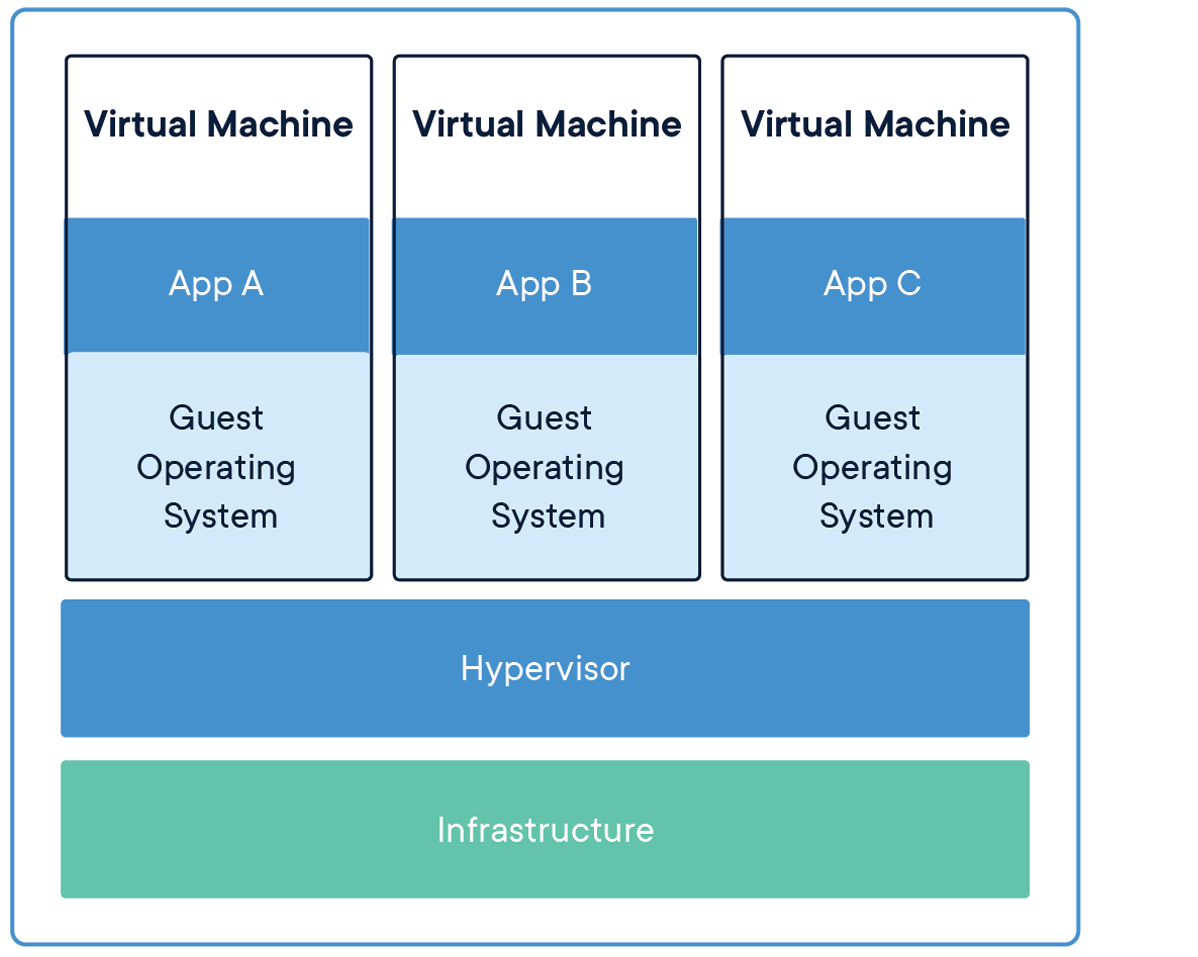
\includegraphics[scale=0.25]{fig/dockercontainer.png}
  \centering
  \caption{Three docker containers sharing the same infrastructure}
  \label{fig:dockercontainer}
\end{figure}

Suppose we have one user (device) and three computing parties (server)\footnote{Note that for ease, we use a loopback interface (localhost)}. We use the terms device and server to differentiate between two groups. On one hand we have the users who request a secure face matching task to be done, these users belong to the device group. On the other hand we have the parties doing the MPC, they belong to the server group.

The parties can be simulated by using three different Docker containers (figure \ref{fig:dockercontainer}), these containers share the same infrastructure (network). By setting the containers to different ports (5000, 5001, 5002 and 11365, 11366, 11367) on this network we can access, the containers from outside (device)\footnote{With outside we mean outside of the other containers, but the machine accessing the containers must still be on the loopback interface}. The Docker file (listing~\ref{lst:docker}) and environment file (listing~\ref{lst:env}) for  setting up the three parties.

\begin{lstlisting}[caption={Docker files for servers}, label={lst:docker}, frame=single]
FROM tsutomu7/scientific-python
MAINTAINER Carlton Shepherd "carlton.shepherd@onespan.com"
COPY . /app

# Install requirements
WORKDIR /app
RUN pip install -r requirements.txt

# Install MPyC from source after giving
# default user (scientist) all ownership
WORKDIR ./mpyc
USER root
RUN chown -R scientist .
USER scientist
RUN python setup.py install --user

#EXPOSE 11365

# Launch server
WORKDIR ../
CMD ["python -u", "./app.py"]
\end{lstlisting}

The \codeword{app.py} script runs a webserver using the python package flask and a database using the python package pymongo (MongoDB). The webserver will be used to communicate between the device and the server (to launch the MPC protocol, clear the database, ...) while the MongoDB will be used to store the secret shares for that particular server.

\begin{lstlisting}[caption={Environment file for servers}, label={lst:env}, frame=single]
N_PARTIES=3
PARTY_0_HOST=localhost
PARTY_0_PORT=5000
PARTY_1_HOST=localhost
PARTY_1_PORT=5001
PARTY_2_HOST=localhost
PARTY_2_PORT=5002
\end{lstlisting}

When all three parties (server) are up and running as can be seen in figure \ref{fig:mpc_shells}, the user (device) can start encrypting their input image containing their face using Shamir's secret sharing scheme (listing \ref{lst:ssss}). The user shares each pixel of the image in to three secret shares, one for each party. The user then sends their three sets of secret shares (encrypted image) to the parties, each party receives only one set of shares.

\begin{figure}[H]
  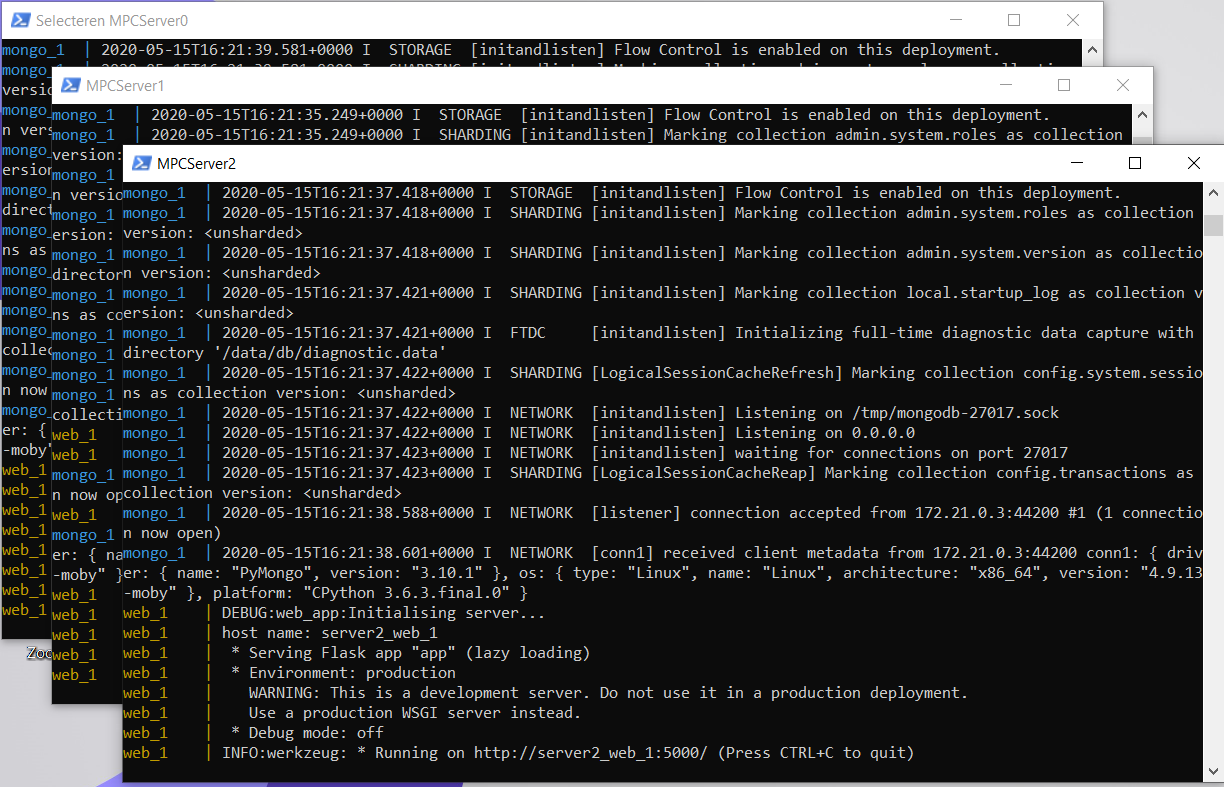
\includegraphics[scale=0.5]{fig/mpc_shells.png}
  \centering
  \caption{Each MPC party has their own interactive shell}
  \label{fig:mpc_shells}
\end{figure}

\begin{lstlisting}[caption={Shamir secret sharing algorithm (part of MPyC framework)}, label={lst:ssss}, frame=single, breaklines=true]
def random_split(s, t, m):
    field = type(s[0])
    p = field.modulus
    order = field.order
    T = type(p) # T is int or gf2x.Polynomial
    n = len(s)
    shares = [[None] * n for _ in range(m)]
    for h in range(n):
        c = [secrets.randbelow(order) for _ in range(t)]
        # polynomial f(x) = s[h] + c[t-1] x + c[t-2] x^2 + ... + c[0] x^t
        for i in range(m):
            y = 0 if T is int else T(0)
            for c_j in c:
                y += c_j
                y *= i + 1
            shares[i][h] = (y + s[h].value) % p
    return shares
\end{lstlisting}

The algorithm above splits each secret given by parameter s (list of secrets) into m random Shamir shares. The degree for the Shamir polynomials is t remember  $0 \leq t < n$. The algorithm returns a matrix of shares, one row per party.\\

Finally the user can start the computation by, sending a the appropriate request to one of the parties (listing \ref{lst:devicelaunch}). We make use of the requests package, requests is a simple HTTP library for python it enables us to make requests and get responses over HTTP.

\begin{lstlisting}[caption={Sending request for secure face matching task}, label={lst:devicelaunch}, frame=single, breaklines=true]
# Define hosts and ports
hosts = ['localhost', 'localhost', 'localhost']
ports = [5000, 5001, 5002]

# Shares secrets
image = cv2.imeread("face.pgm")
kernel = [[1,1,1],[0,0,0],[-1,-1,-1]]
send_shares_mpc(image, ['Image'], 'test', hosts, ports, combined = True)
send_shares_mpc(kernel, ['Filters'], 'model', hosts, ports, combined = True)

# Start MPC
url = f'http://{hosts[0]}:{ports[0]}/mpyc_launch?api=face_matching_server'
response = requests.get(url)
# Response contains output of the MPC
\end{lstlisting}

Note that the HTTP response we get from the GET request contains two variables; the status code and the text. The status code indicates wheter the HTTP request has been  succesfully completed, a valid and succesfull request has a response code of 200. The text of a response is the message that is transferred in the body of the HTTP response. We use the HTTP as means of communication between the device and the server. Note that for more secure implementations, HTTPS (Hypertext Transfer Protocol Secure) is preferred. Since traffic in HTTPS is encrypted using Transport Layer Security (TLS). Using HTTPS denies MITM attacks (man-in-the-middle), a type of attack where a passive attacker tries to eavesdrop certain packets of the traffic.\\

The GET query of the request sent in listing \ref{lst:devicelaunch} executes the following code (listing \ref{lst:mpyclaunch}) on the first party or PARTY\_0 (localhost:5000).

\begin{lstlisting}[caption={Launching MPC and returning formatted output}, label={lst:mpyclaunch}, frame=single, breaklines=true]
is_running = False
@app.route("/mpyc_launch", methods=["GET"])
def mpyc_launch():

    def get_api_name(api_name):
        return api_name + '.py'

    http_arg = request.args.get('api')
    script_name = get_api_name(http_arg)
    if script_name is None:
        return "400"

    os.chdir(main_wd)
    test_path="./mpyc/demos"
    os.chdir(test_path)
    # Raise other parties
    Party = os.getenv(f"Party")
    # Only execute following code for PARTY_0
    if Party == '0':
        global is_running
        if is_running:
            return '200'
        else:
            is_running = True

        for i in range(int(os.getenv('N_PARTIES')) - 1, 0, -1):
            party_host = os.getenv(f'PARTY_{i}_HOST')
            party_port = os.getenv(f'PARTY_{i}_PORT')
            host_addr = f'http://{party_host}:{party_port}/mpyc_launch?api={http_arg}'
            r = requests.get(host_addr)
            time.sleep(2.50)

        # Run MPC script (PARTY_0)
        process = subprocess.Popen(['python', script_name, '-c', f'party{3}_0.ini'], stdout=subprocess.PIPE)
        stdout, stderr = process.communicate()
        is_running = False

        # Output everything inside of the '$$$' tags
        output_formatted = stdout.decode().split('$$$')[1]
        output_formatted = output_formatted.split('$$$')[0]
        output_formatted = output_formatted.strip()
        output_formatted = output_formatted.replace('\n', '')
        output_formatted = output_formatted.strip(',')
        return output_formatted

    else:
        # Run MPC script (party_1 and party_2)
        os.system(f'python {script_name} -c party{3}_{Party}.ini &')
        return "200"
\end{lstlisting}

The value of the api argument from the GET request determines which MPC script gets excecuted. Then PARTY\_0 starts executing the same code snippet (mpyc\_launch) on the other two parties, by sending the appropriate requests. The first party then executes a new subprocess that runs a the MPC script. The result of the MPC script gets written to the STDOUT stream (standard output) which can be read by the parent process. The result gets parsed in the MPC script, by printing the result between two \$\$\$ tags (like this \$\$\$ result \$\$\$). The other two parties skip most of the code (because their environment variable 'Party' differs from 0) and go straight to executing the same MPC script. Notice that PARTY\_0 plays an important role in establishing that the MPC script runs on the other parties. This centralisation is a clear weakness of this implementation, because a corrupted PARTY\_0 could cause great harm to the correctness of the protocol. But for the sake of simplicity we opt for this more centralised implementation. An overview of this implementation with the different groups (device and server) can be seen in figure \ref{fig:implementationoverview}.

\begin{figure}[H]
  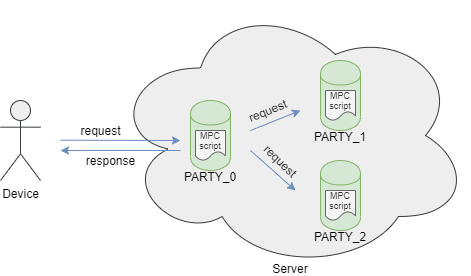
\includegraphics[scale=0.75]{fig/implementationoverview.png}
  \centering
  \caption{Overview of MPC implementation over HTTP (3 parties)}
  \label{fig:implementationoverview}
\end{figure}

Last but not least, we discuss the mpc script that needs to run on the three parties. This script does the actual MPC. Each party holds an identical copy of this script. The parties begin by opening connections with each other (\codeword{mpc.start}). Remember: parties need to communicate with each other in order to output a result or to do non-linear operations such as multiplication of two secure numbers. Then the parties load the unique secret shares for the image and the convolution kernels stored in their MongoDB databases. Since the secret shares are stored in lists in the database, the parties reshape them to the original shape. Then the parties securely compute an output for the input image and kernels on a series of sequential layers (convolution, max pooling and ReLU) made out of the essential building blocks we introduced at the beginning of this chapter. Finally the parties output the result (\codeword{mpc.output}) print the result (printing in python has the same effect as writing to STDOUT) but they do this in a manner such that the stream is parsed. Note that all parties print the result, but only PARTY\_0's STDOUT will be looked at. This is yet another flaw of our implementation. Better would be to look at everybody's STDOUT, to check if anyone is cheating by printing something other than the true result. Finally the parties begin shutting down (mpc.shutdown), closing all open connections. The subprocess will exit, unpausing the parent process. Which will unparse the STDOUT and return the result as a response to the device.\\

 A basic example of an mpc script that contains all of the points made earlier can be observed in listing \ref{lst:mpcscript}.

\begin{lstlisting}[caption={Example of MPC script for a single CNN layer (conv,maxp and relu)}, label={lst:mpcscript}, frame=single, breaklines=true]
import math
import numpy as np
from mpyc.runtime import mpc
from load_database import load_data
from custom_operations import convolution, relu, maxpool

async def main():
    await mpc.start()

    images = load_data('Image', 'test')
    kernels = load_data('Filters', 'model')
    image = images[0]
    kernel = kernels[0]

    image = np.reshape(image, (int(math.sqrt(len(image))), int(math.sqrt(len(image)))))
    kernel = np.reshape(kernel, (int(math.sqrt(len(kernel))), int(math.sqrt(len(kernel)))))

    conv = convolution(image, kernel)
    maxp = maxpool(conv)
    result = relu(maxp)
    result = list(np.asarray(result).flatten())

    print("$$$\n")
    print(await mpc.output(result))
    print("$$$")

if __name__ == '__main__':
    mpc.run(main())
\end{lstlisting}

Obviously a CNN has way more layers than just this triplet (convolution, max pooling and ReLU). But we will discuss the secure design of the CNN later on in chapter \ref{SecureCNN}.

\section{Design}
\label{Design}
In this chapter we discuss how we designed the neural network and why we chose for the network's architecture in specific. After explaining the neural network's architecture, we will have a look at how we translate a model working on plaintext pictures, to a secure model using MPC.

\subsection{Convolutional Neural Network Architecture}
\label{ConvolutionalNeuralNetworkArchitecture}
In the process of choosing the best architecture for a CNN, we found four suitable models. We will see how each of these models are designed and in what way they differ from the others. Finally, we select one of these models to make it secure using MPC, the selection depends on the following criteria; straightforwardness of the MPC implementation, size of the network (number of parameters), accuracy of the model and the preferred output (distance vector or binary classification).\\

\textbf{General (applies for all models):} The input dimensions of the different neural networks is the same (1 x 100 x 100). The output can differ depending on what loss function is used (cross entropy loss or contrastive loss), but the meaning is the same, wheter a face matches another face or not. And the only difference is how to differentiate between these two classes (match or no match), this means the arbitrary threshold must be chosen on a different basis. To choose a good threshold that reflects the accuracy of the model, we iterate the calculation of the precision and recall for each threhold value in a certain range. This gets us the following curve (figure \ref{fig:threshold}), out of which we can distract the best threshold.\\

\begin{figure}[H]
  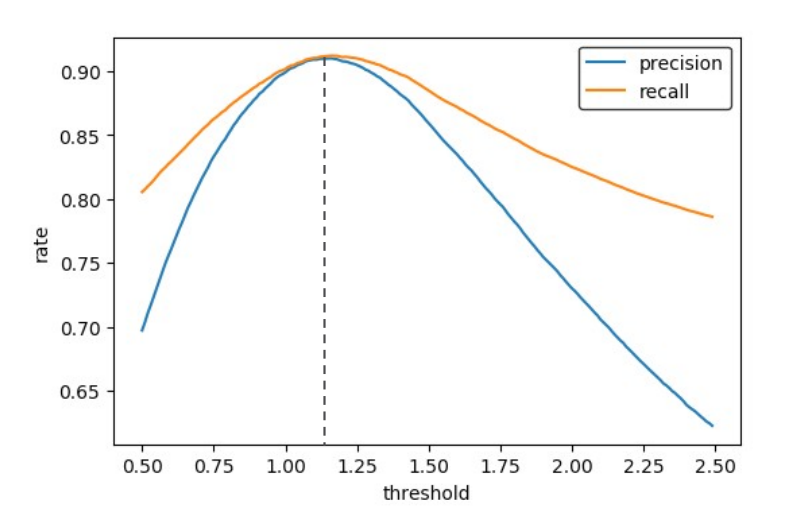
\includegraphics[scale=0.6]{fig/threshold.png}
  \centering
  \caption{Curve for selecting the best threshold value}
  \label{fig:threshold}
\end{figure}

\textbf{CNN with Contrastive Loss:} This model is the first model we designed. It is simple and basic yet powerful. The neural network design can be seen in figure \ref{fig:ccncl}.

\begin{figure}[H]
  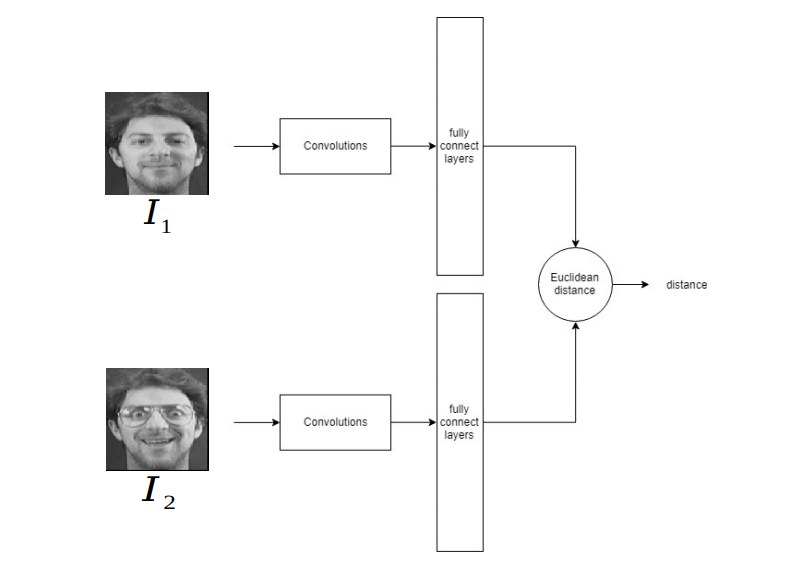
\includegraphics[scale=0.7]{fig/cnncl.png}
  \centering
  \caption{CNN with Contrastive Loss function}
  \label{fig:ccncl}
\end{figure}

The convolution layers, including Max-pooling (2 x 2 with stride 2) and ReLU after every convolution, consist out of four layers:

\begin{enumerate}
  \item 4 convolutions (7 x 7).
  \item 8 convolutions (5 x 5).
  \item 16 convolutions (3 x 3).
  \item 32 convolutions (3 x 3).
\end{enumerate}

Each of these layers have different tasks. The first layers have larger convolution filters, these convolutions detect high-level features like distance or rotation between ears, nose and/or eyes. While the latter, smaller convolution filters detect low-level features like lines or dots (jawline, eyes, mouth).

After the final convolution layer we flatten the output layer to a one-dimensional tensor. This tensor then serves as input for a small fully connected neural network (perceptron), this network can be seen as an extension of the CNN. We use this fully connected neural network to add global spatial correlation (a CNN is good for recognizing structures in local and neighbouring pixels). Since it's important to also important that the algorithm detects two objects or features that belong to each other even though they are seperated and are not local or neighbouring, think of two ears on a face for instance.\\

The total number of learnable parameters (weights and biases) in this neural network is 154.592, the model doesn't show any sign of overfitting nor underfitting up to 500 epochs.\\

The code for this neural network is printed in below (listing~\ref{lst:cnncl}). Notice how simple this neural network is. With only four convolutional layers, it is able to make a face matching decision.

\begin{lstlisting}[caption={Code for CNN with Contrastive Loss}, label={lst:cnncl}, frame=single, breaklines=true]
class SiameseNetwork(nn.Module):
    def __init__(self):
        super(SiameseNetwork, self).__init__()

        self.cnn1 = nn.Sequential(
            nn.Conv2d(1, 4, kernel_size=7),
            nn.MaxPool2d(kernel_size=2, stride=2, padding=0),
            nn.ReLU(),
            nn.Conv2d(4, 8, kernel_size=5),
            nn.MaxPool2d(kernel_size=2, stride=2, padding=0),
            nn.ReLU(),
            nn.Conv2d(8, 16, kernel_size=3),
            nn.MaxPool2d(kernel_size=2, stride=2, padding=0),
            nn.ReLU(),
            nn.Conv2d(16, 32, kernel_size=3),
            nn.MaxPool2d(kernel_size=2, stride=2, padding=0),
            nn.ReLU(),
        )

        self.fc1 = nn.Sequential(nn.Linear(512, 256), nn.ReLU(), nn.Linear(256, 64))

    def forward_once(self, x):
        output = self.cnn1(x)
        output = output.view(output.size()[0], -1)
        output = self.fc1(output)
        return output

    def forward(self, input1, input2):
        output1 = self.forward_once(input1)
        output2 = self.forward_once(input2)
        return output1, output2
\end{lstlisting}

\textbf{CNN with Cross Entropy Loss:} The following model (figure \ref{fig:cnncel}) is similar to the first one we described earlier. The key differences of this model, is that the siamese neural network stops after the last layer. The two output layers get flattened to two single one-dimensional tensors. These tensors then get concatenated. The concatenated tensor now gets sent trough a single fully connected neural network (perceptron).\\

\begin{figure}[H]
  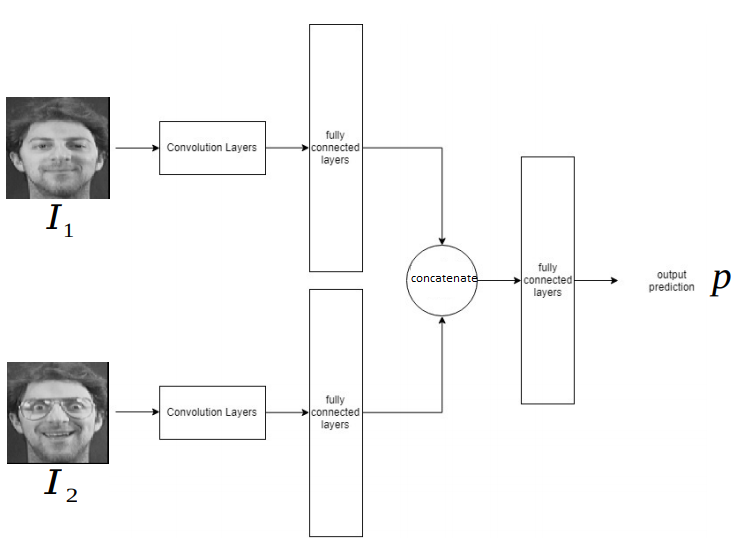
\includegraphics[scale=0.7]{fig/cnncel.png}
  \centering
  \caption{CNN with Cross Entropy Loss function}
  \label{fig:cnncel}
\end{figure}

 Note that in the first model (CNN with Contrastive Loss) there is no fusion of the siamese neural network. And the only time the two inputs depend on each other, is when we calculate the euclidean distance between the two output tensors. In fact, this type of model is not really a pure siamese neural network anymore. We guess that the perceptron, placed after the convolution layers, performs some sort of comparison on the two output tensors and we hope this comparison will be better than the standard euclidean distance.\\

 Finally, the cross entropy loss is calculated on the last layer of the model. Since face matching is a binary task (matching or not matching), the last layer contains a single neuron (class). The cross entropy of that neuron returns the chance for that class to be true. The pleasant advantage of cross entropy is that we don't have to set up an arbitrary threshold value, the threshold is simply already decided, for instance if $p \in [0,1]$ than the threshold is equal to $p = 0.5$. If two faces are simmilar, $p=0$. If two faces are dissimilar, $p=1$.\\

 The convolution layers consist of the same number of convolutions, as the first model:

 \begin{enumerate}
   \item 4 convolutions (7 x 7).
   \item 8 convolutions (5 x 5).
   \item 16 convolutions (3 x 3).
   \item 32 convolutions (3 x 3).
 \end{enumerate}

 The code for the model is listed below (listing~\ref{lst:cnncel})

 \begin{lstlisting}[caption={Code for CNN with Cross Entropy Loss}, label={lst:cnncel}, frame=single, breaklines=true]
 class SiameseNetworkConcat(nn.Module):
    def __init__(self):
        super(SiameseNetwork, self).__init__()

        self.cnn1 = nn.Sequential(
            nn.Conv2d(1, 4, kernel_size=7),
            nn.MaxPool2d(kernel_size=2, stride=2),
            nn.ReLU(),
            nn.Conv2d(4, 8, kernel_size=5),
            nn.MaxPool2d(kernel_size=2, stride=2),
            nn.ReLU(),
            nn.Conv2d(8, 16, kernel_size=3),
            nn.MaxPool2d(kernel_size=2, stride=2),
            nn.ReLU(),
            nn.Conv2d(16, 32, kernel_size=3),
            nn.MaxPool2d(kernel_size=2, stride=2),
            nn.ReLU(),
        )

        self.fc1 = nn.Sequential(
            nn.Linear(1600, 100), nn.ReLU(inplace=True), nn.Linear(100, 10),
        )

        self.fc2 = nn.Sequential(
            nn.Linear(20, 20), nn.ReLU(inplace=True), nn.Linear(20, 1),
        )

    def forward_once(self, x):
        output = self.cnn1(x)
        output = output.view(output.size()[0], -1)
        output = self.fc1(output)
        return output

    def forward(self, input1, input2):
        output1 = F.relu(self.forward_once(input1))
        output2 = F.relu(self.forward_once(input2))
        output = torch.cat((output1, output2), dim=1)
        output = self.fc2(output)
        return output
 \end{lstlisting}

\textbf{Residual Neural Network:} The last model makes use of a special type of deep learning, known as deep residual learning, introduced in 2015 by \cite{he2016deep}. A Residual Neural Network (ResNet) is a special type of neural network that utilizes shortcuts or skip connections shortcuts to jump over a number of layers. Neural networks implementing residual blocks (figure \ref{fig:residualblock}) can have way more layers without running in to problems like vanishing gradient. Vanishing gradient problem occurs when certain parameters of a network do not get updated during training, because the gradient will be so small that it will prevent the parameters from changing. With ResNet a direct link (identy function) can be found over multiple layers, thus creating a way to link certain inputs deeper into the network.

\begin{figure}[H]
  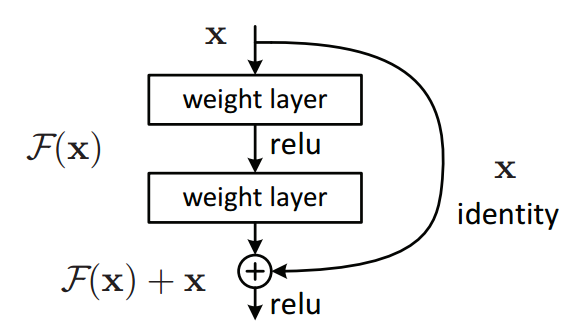
\includegraphics[scale=0.5]{fig/residualblock.png}
  \centering
  \caption{Residual block (2-layer skipping)}
  \label{fig:residualblock}
\end{figure}

In short, ResNet allows us to use way more layers than before. So we derived our own ResNet-like model, from the pre-trained ResNet models available from Pytorch \footnote{\url{https://github.com/pytorch/vision/blob/master/torchvision/models/resnet.py}}. We saw an incline in accuracy using ResNet, but with more layers, there are more parameters and the complexity rises.

A basic residual block can be coded in Pytorch in the following way (\ref{lst:residualblock})

\begin{lstlisting}[caption={Pytorch Code for Residual Block}, label={lst:residualblock}, frame=single, breaklines=true]
class BasicBlock(nn.Module):
    def __init__(self, in_planes, planes, stride=1):
        super(BasicBlock, self).__init__()
        self.expansion = 1
        self.conv1 = nn.Conv2d(in_planes, planes, kernel_size=3)
        self.bn1 = nn.BatchNorm2d(planes)
        self.conv2 = nn.Conv2d(planes, planes, kernel_size=3)
        self.bn2 = nn.BatchNorm2d(planes)
        self.pool = nn.MaxPool2d(2,2)

        self.shortcut = nn.Sequential()
        if stride != 1 or in_planes != self.expansion*planes:
            self.shortcut = nn.Sequential(
                nn.Conv2d(in_planes, self.expansion*planes, kernel_size=1, stride=stride, bias=False),
                nn.BatchNorm2d(self.expansion*planes)
            )

    def forward(self, x):
        out = F.dropout(F.relu(self.bn1(self.conv1(x))), p=0.3)
        out = self.bn2(self.conv2(out))
        out += self.shortcut(x)
        out = F.relu(out)
        return out
\end{lstlisting}

Notice that the \codeword{self.shortcut} function is simply the identity function.\\

As we said before choosing a neural network depends on a number of factors, we will now rank each of the neural networks described above for each determining factor.\\

Starting with the straightforwardness of the MPC implementation, in other words, how easy will it be to translate the code written with Pytorch to a MPC algorithm using no libraries for neural networks (since Pytorch doesn't support secure datatypes). It's obvious that a ResNet architecture requires more attention to detail and is more complex to implement. The other two neural networks require less attention to detail, thus are more easy to implement.\\

Next, we compare size of the neural network. The neural network's size or it's number of parameters is an equally important factor. Since MPC protocols are way slower than classic computations. We would like our neural network to do fast computations. Fast computations corresponds to less computations, and less computations corresponds to less (or smaller) convolutions or fully connected layers. Thus we would like our network to have a small number of layers, but still enough to be able to differentiate between faces. Since ResNet only adds extra layers, this model is again not preffered. The other two models have about the same number of parameters, and only the fully connected layers have a different number of weights and biases.\\

Ranking the neural networks on accuracy (the ability to match faces) was done by testing the four different networks, the results can be seen in table \ref{table:designaccuracy}. We find that when we are using the Contrastive Loss function, the classic CNN as well as the ResNet model is giving us better results than with the Cross Entropy loss function. Overall the ResNet model has a slightly better accuracy than the classic CNN.


\begin{table}[H]
\centering
\begin{tabular}{||c c c||}
 \hline
 Model & Loss & Accuracy \\ [0.5ex]
 \hline\hline
 Classic CNN  & Contrastive Loss & 89.20\% \\
 Classic CNN  & Cross Entropy Loss & 81.94\% \\
 ResNet (8 layers)  & Contrastive & 91.06\% \\
 ResNet (8 layers)  & Cross Entropy Loss & 84.13\% \\
 \hline
\end{tabular}
\caption{Accuracy of the different models}
\label{table:designaccuracy}
\end{table}

Last but not least, what output do we prefer? The models with Contrastive loss have an output in the form of a score, the distance between two output vectors gets calculated. While the models with Cross Entropy loss simply output a chance, not having to worry about choosing a certain threshold. During the testing of the networks we argued that determining the threshold is not too hard, in fact the threshold can be easily chosen by drawing out a graph of the accuracy of the network and the different thresholds as in figure \ref{fig:ccncl}.\\

Taking every factor in to consideration, we concluded that a classic CNN with Contrastive Loss offers a high enough accuracy and low complexity, while still being easy to implement in MPC.\\

\subsection{Secure CNN}
\label{SecureCNN}
In the following part of this chapter we will discuss specifically what parts of the classic CNN we will encrypt. We ask ourselves the question: After how many convolution layers, ReLU layers and max pooling layers will the output be unrecognizable?\\

 Suppose that the activations after the first $n$ layers can not be traced back to the face present on the input image, then we don't need to encrypt the whole CNN but only the first $n$ layers. We could split up the neural network in two parts; a part that is encrypted and uses MPC to do certain operations and a part that is unencrypted. Of course the encrypted part must be placed before the unencrypted part. Otherwise the face would not be encrypted.

\begin{figure}[H]
  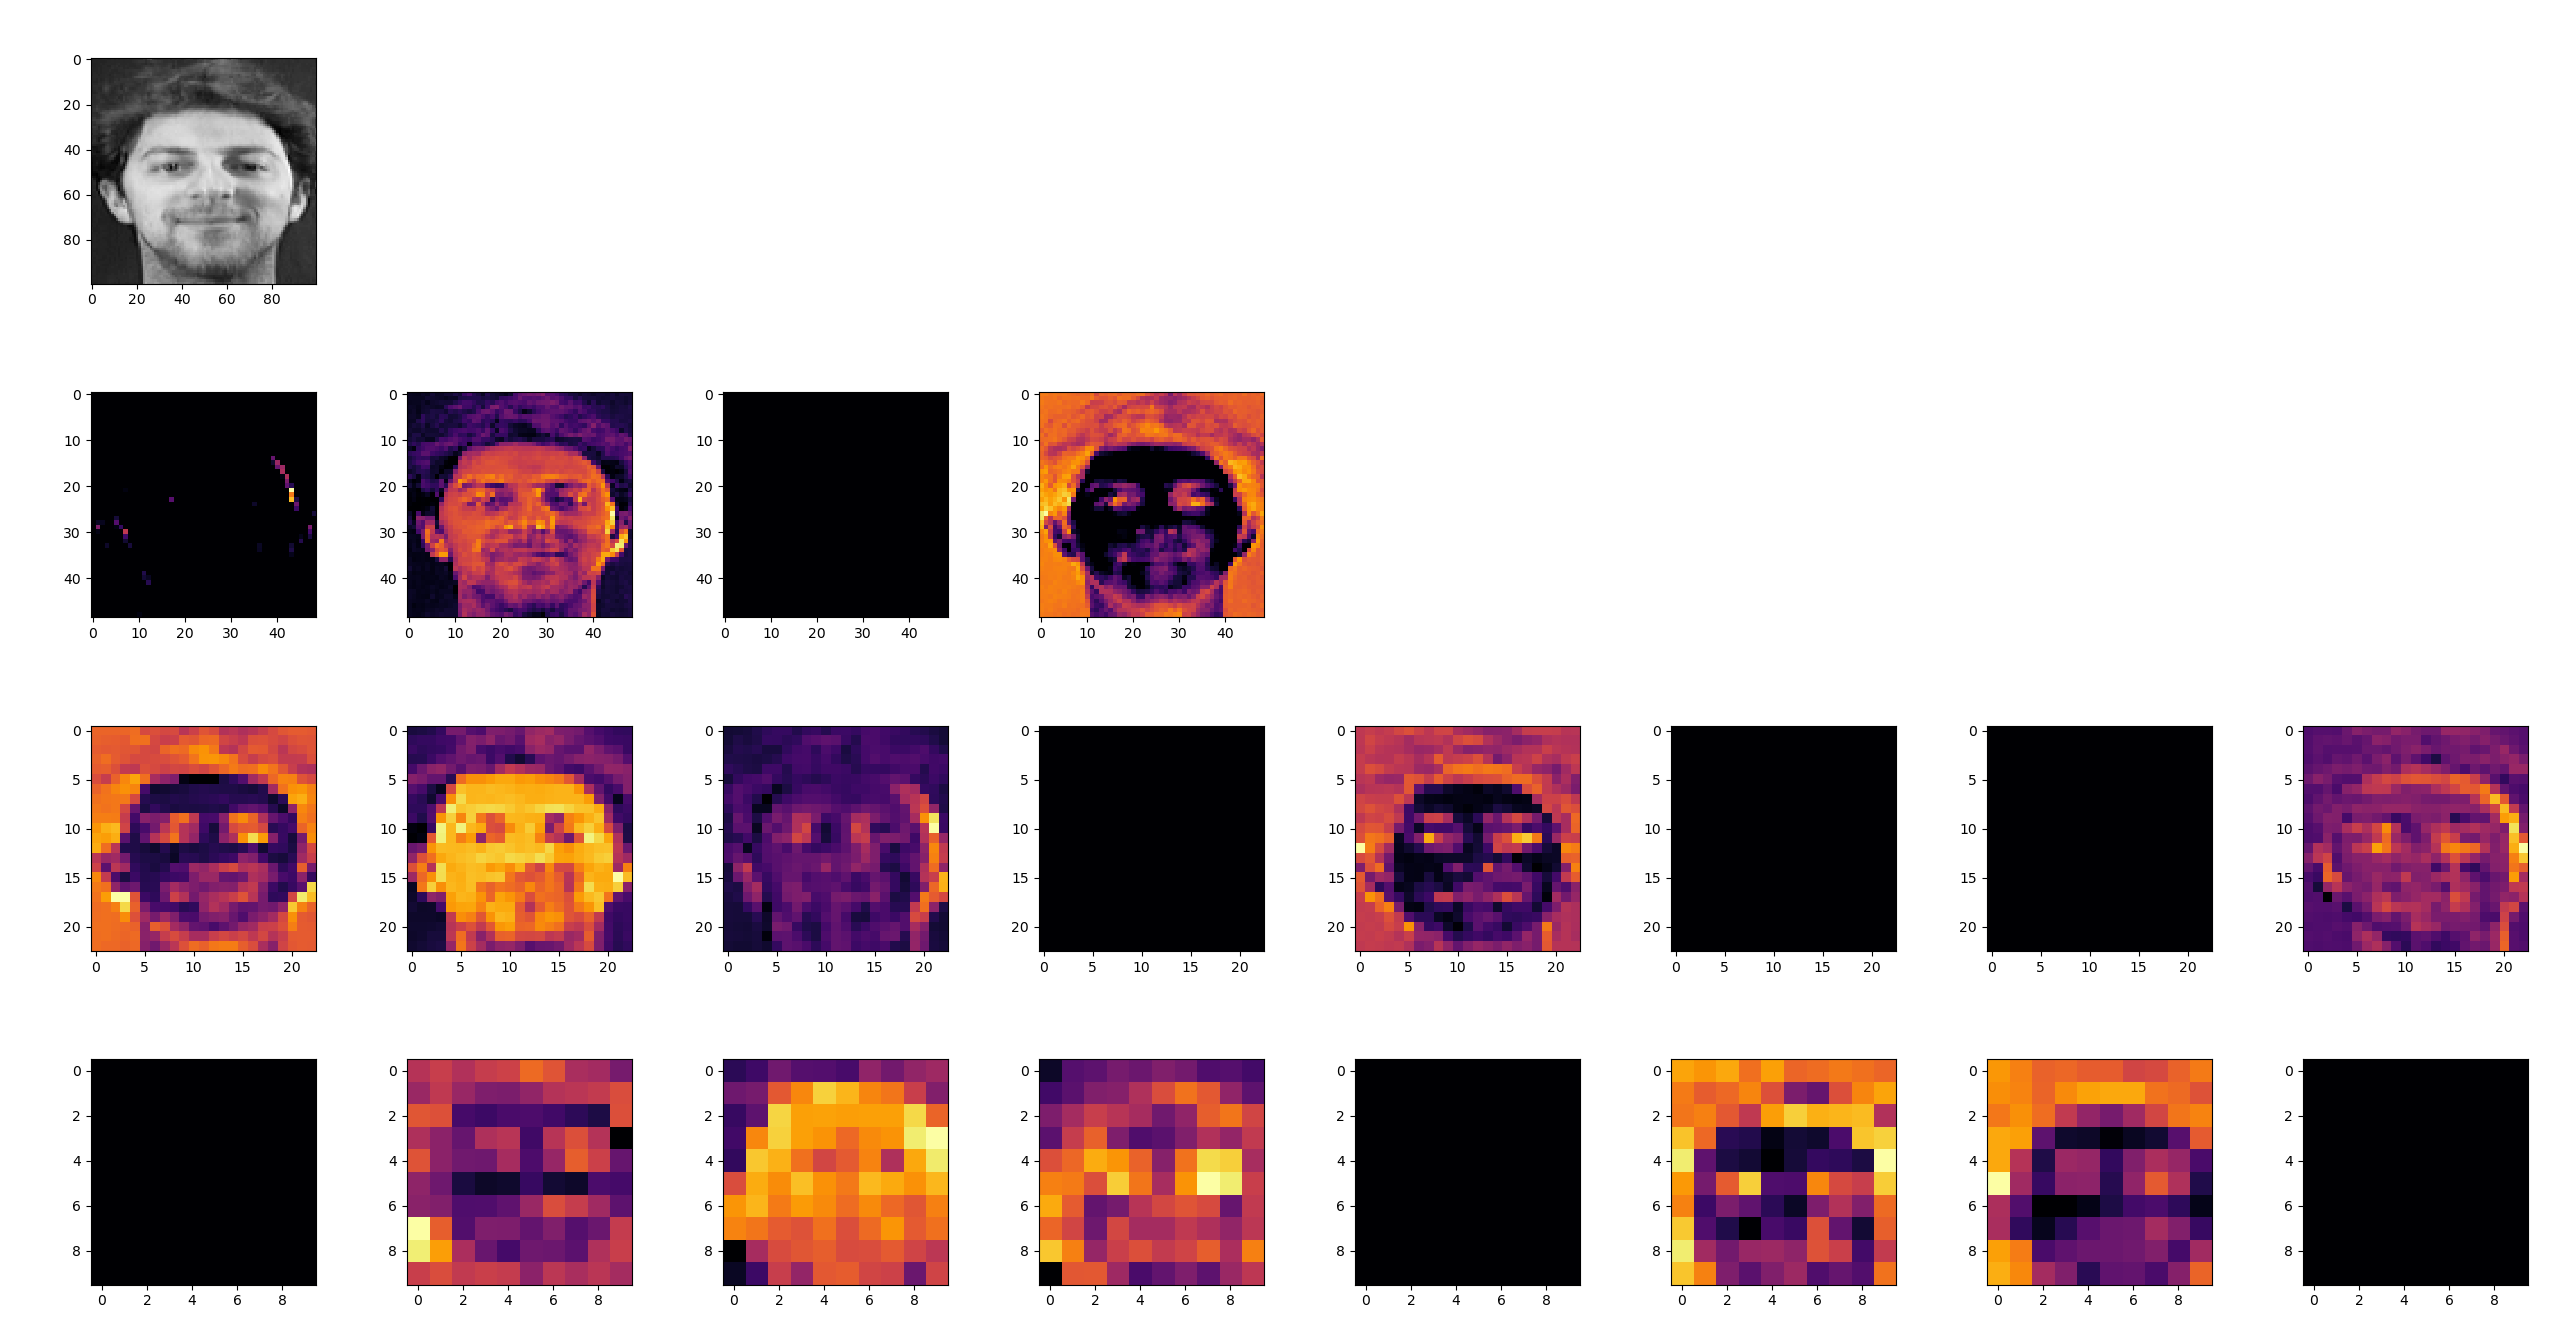
\includegraphics[scale=0.2]{fig/activations/7.png}
  \centering
  \caption{All Activation maps for an image}
  \label{fig:activations}
\end{figure}

An activation map or feature map is the hidden output activations for a given convolution filter. They are called activation/feature maps because you can clearly see features or certain areas in the output that are more important than others (high activations). Activation maps give an insight to what features the CNN extracts from the input. In figure \ref{fig:activations} an overview of all the activation maps for a certain image can be seen. The first image is the input. The four pictures below that are activation maps of the first layer. The eight pictures below those are the activation maps from the second layer. And the last eight pictures are the activation maps from the last layer.

\begin{figure}[H]
  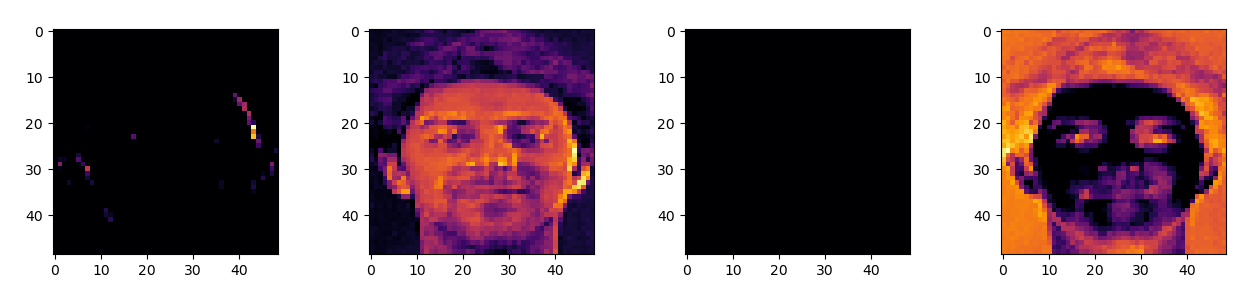
\includegraphics[scale=0.4]{fig/activations/7_1.png}
  \centering
  \caption{Activation maps after the first layer}
  \label{fig:activation_1}
\end{figure}

As you can see in figure \ref{fig:activation_1} the activation maps after the first layer are not obfuscated enough and can be recognized fairly easily by machines or humans. Thus only encrypting this part of the CNN would not be sufficient for a privacy preserving face matching algorithm. Notice how the resolution of the image became twice as small (this effect is caused by max pooling) and is thereby much more difficult to recognize. Another perturbation that is taking place is the ReLU activation function, discarding all negative values from the output. Lastly the convolutions can cause small to great perturbations to the image depending on the convolution filter.

\begin{figure}[H]
  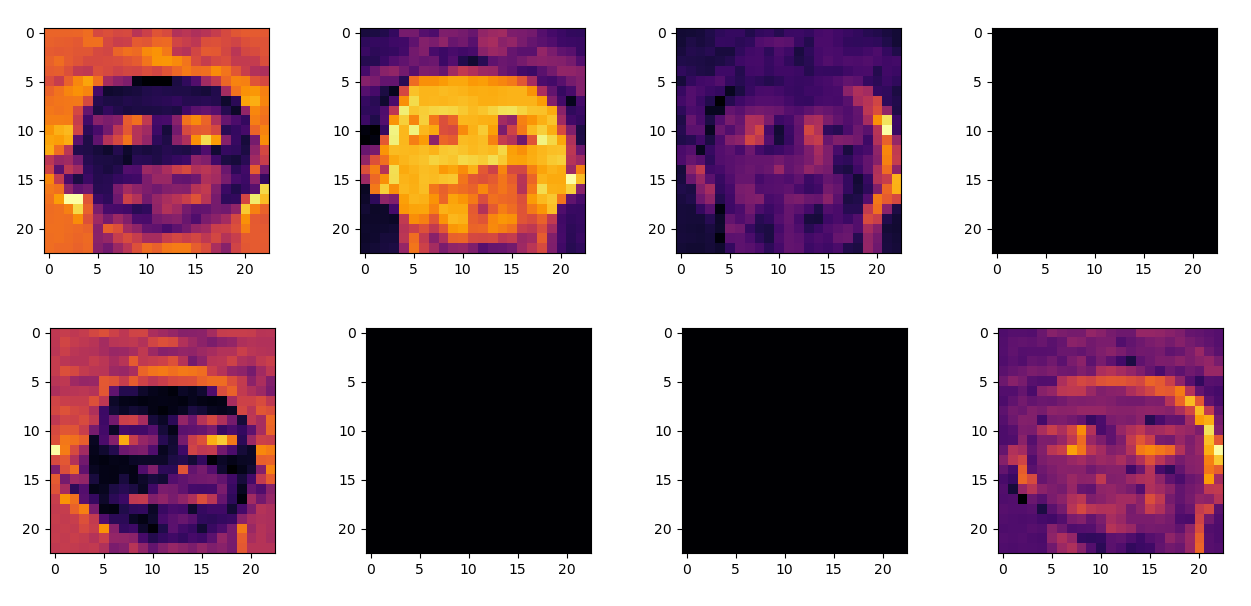
\includegraphics[scale=0.4]{fig/activations/7_2.png}
  \centering
  \caption{Activation maps after the second layer}
  \label{fig:activation_2}
\end{figure}

The activation maps after the second layer (figure \ref{fig:activation_2}) are very pixelated. But since we can still recognize some major facial features, like the hair and the shape of the face. So this part of the neural network should still be encrypted.

\begin{figure}[H]
  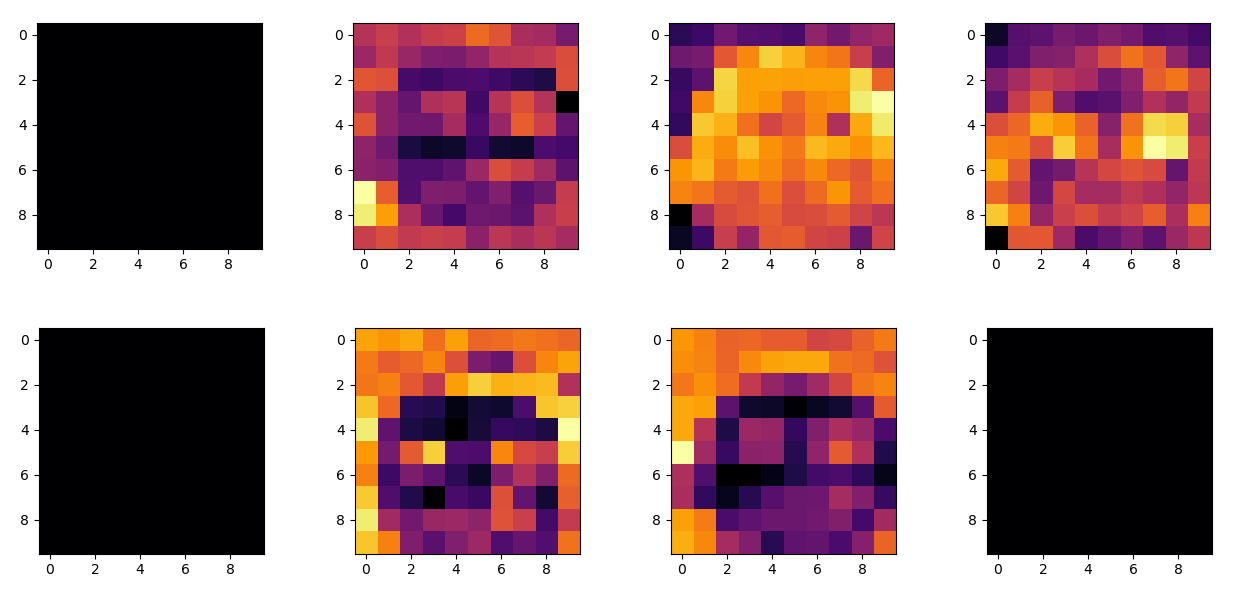
\includegraphics[scale=0.4]{fig/activations/7_3.png}
  \centering
  \caption{Activation maps after the third layer}
  \label{fig:activation_3}
\end{figure}

Finally, we observe that it is impossible to recognize a face in one of the activation maps after the third layer (figure \ref{fig:activation_3}). The activation map is so pixelated that we can not recognize anything in it. Therefore we could make the third layer and everything that comes after it part of the unencrypted neural network. So that only the first two layers of the CNN needs to be encrypted using MPC. Of course for additional security one may choose to encrypt more than only the first two layers or even the whole neural network. But keep in mind that opting for more security by encrypting more layers, comes with an additional cost in complexity. We call this the security-complexity tradeoff.\\

The attentive reader may have noticed that certain of these activation maps are entirely black or predominantly black, if not have a look at figure \ref{fig:pruning_before}, meaning they don't contain any information or are useless. We realized that this phenomenon was occuring on the same activation map for every single image which inferred through the CNN. The convolution filter's weights were close to zero or negative, this meant that any input to those specific convolutions would have an output close to zero or negative. In fact this is not really a problem but after the ReLU activation layer all of the values of the activation map would be equal to zero. Rendering the activation map and the convolution as a whole obsolete. To take an advantage of this we used some form of pruning.

\begin{figure}[H]
  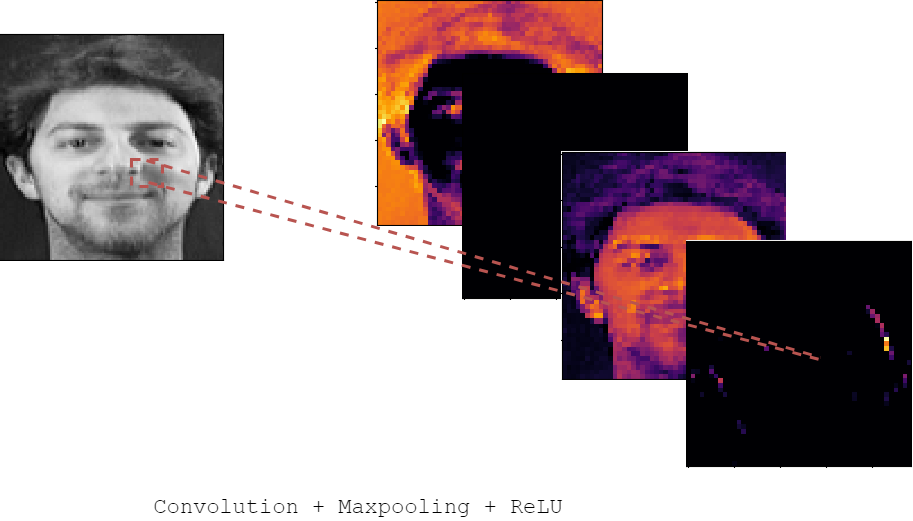
\includegraphics[scale=0.4]{fig/pruning_before.png}
  \centering
  \caption{First layer without pruning}
  \label{fig:pruning_before}
\end{figure}

Pruning is a technique in machine learning that enables neural networks to be more efficient. It's an optimization technique that cuts out any unnecessary weights or biases. The result is a compressed, smaller version of the neural network than before, making it faster and less complex. There exists different processes and pipelines for pruning, and often neural networks are given too much parameters on purpose to apply pruning later on.

In our case we can safely remove any of the convolutions causing the activation map to turn out black. And without losing too much accuracy we can also remove any convolution filter that doesn't provide enough information and is deemed insufficient. The following figure \ref{fig:pruning_after} displays how the first layer only outputs two activation maps after pruning, instead of the four activation maps that were produced in the original CNN.

\begin{figure}[H]
  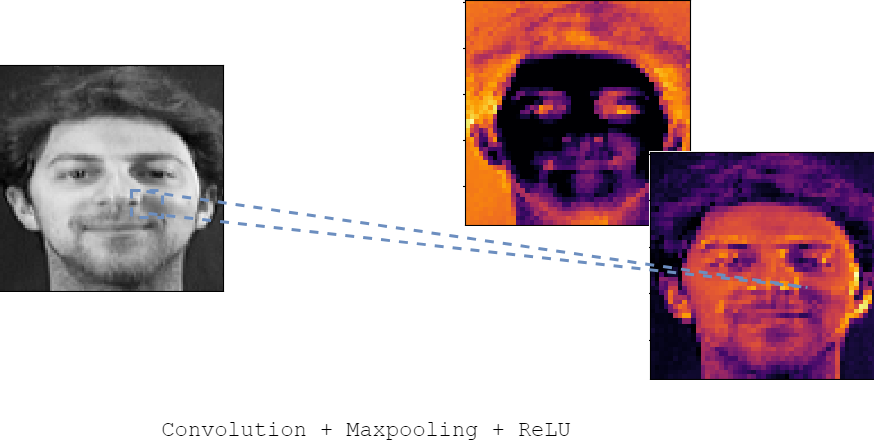
\includegraphics[scale=0.4]{fig/pruning_after.png}
  \centering
  \caption{First layer after pruning}
  \label{fig:pruning_after}
\end{figure}

Eight out of the twenty convolution filters are infected with this defect, thus can be ignored or even removed from the CNN. This is great news, since this means we are able to optimize the convolutional part of the CNN with a speedup of around 40\%.\\

Now it is really important that we do the same exact operations that lead the same unencrypted/encrypted input to the same unencrypted/encrypted output. To be sure of how each and every operation works in the cleartext version of the face matching algorithm we strictly follow the Pytorch documentation\footnote{\url{https://pytorch.org/docs/stable/nn.html}}. The \codeword{torch.nn.Conv2d(in_channels, out_channels, kernel_size)} method applies a 2D convolution over an input composed of several input planes. This means that it is possible that more than one tensors can serve as input. This is true in our case for each convolution layer except the first one. The method is implemented as equation \ref{eq:nn.conv2d} where $C$ denotes the number of channels, $\star$ is the 2D cross-correlation operator, $H$ is the height of the input planes and $W$ is the width.

\begin{equation} \label{eq:nn.conv2d}
  out(C_{out_j}) = bias(C_{out_j}) + \sum_{k=0}^{C_{in}-1}weight(C_{out_j},k) \star input(k)
\end{equation}

Notice that in our secure implementation of the \codeword{torch.nn.Conv2d(in_channels, out_channels, kernel_size)} we forgot to add biases and we only allow for one input channel. In fact our implementation looks more like a simple cross-correlation operation.

Adding the biases is really simple. And in fact we can just add the bias to each element of the output by defining a new method \codeword{add_bias(tensor, bias)} (listing~\ref{lst:add_bias}). This method takes two argument; a 2D tensor and a single floating-point bias.

\begin{lstlisting}[caption={Code for adding bias to matrix}, label={lst:add_bias}, frame=single, breaklines=true]
def add_bias(tensor, bias):
    return np.add(tensor, bias)
\end{lstlisting}

The only difference that remains, is that the secure convolution function must allow a combination of input planes. To accomodate for this feature, we define a new method \codeword{conv2d(input, kernel, bias)} that computes the exact same output tensor as the vanilla Pytorch 2D convolution function with only one difference, it being fully encrypted. Notice that we make use of earlier defined methods.

\begin{lstlisting}[caption={Code for computing total 2D convolution}, label={lst:conv2d}, frame=single, breaklines=true]
def conv2d(inputs, kernel, bias):
    output = convolution(inputs[0], kernel)
    for i in range(1, len(inputs)):
        output += convolution(inputs[i], kernel)
    add_bias(output, bias)
    return output
\end{lstlisting}

For the remaining parts of this thesis, when we talk about one convolution we imply the algorithm stated above (listing~\ref{lst:conv2d}), except when clearly stated.

Of course the convolution needs to be done for each convolution filter on the apropriate set of inputs and in the correct order. Just as in the cleartext algorithm (listing \ref{lst:cnncl}), the convolutions are directly followed by the max pooling layers, which are in turn, followed by the ReLU activation layers. With the help of the three main building blocks of the secure CNN we can build convolutional part of the CNN. The other part, which entails the fully connected layers, doesn't need to be encrypted, since it is nearly impossible to recognize someone from a one dimensional tensor of activations, even with knowledge of the parameters of the neural network. Thus, this latter part can be computed on only one of the three servers or on the clients device. The calculation of the euclidean distance between the two output tensors must be done on the client's device, because this way the fingerprint (output tensor) of the validation face (the face of the image that we would like to match).\\

The secure face matching algorithm thus exists out of two parts. The first $n$ encrypted layers make up the first part. The second part includes the rest of the convolutions for which the input tensors are deemed unrecognizable and the fully connected layers. The second part can be computed in the classical way on one of the three servers. MPC is only needed for the first part of the algorithm. This heavily reduces the complexity without compensating for security or privacy.

\begin{figure}[H]
  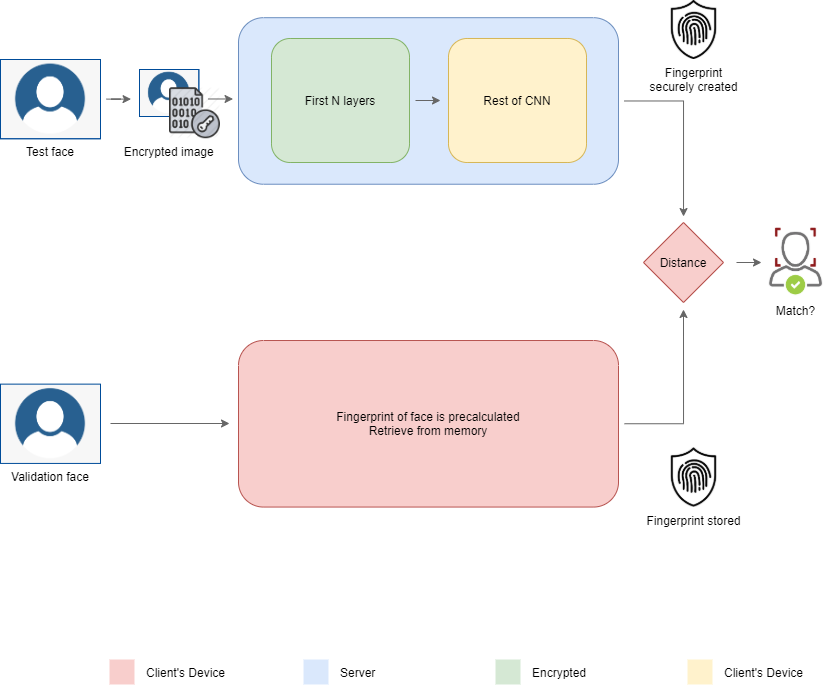
\includegraphics[scale=0.5]{fig/implementation_overview.png}
  \centering
  \caption{Overview of practical implementation of secure face matching algorithm}
  \label{fig:implementation_overview}
\end{figure}

Our secure face matching algorithm still isn't complete. For a match to be succesfull a test image needs to be matched to a validation image (or base image). We could calculate the embedding (fingerprint) of this validation image for each face matching task by inferring the image through the CNN. But the result would always be the same, since the input doesn't change. Therefore it is sufficient to calculate the fingerprint of the image once and store it for a certain period on the client's device. If the fingerprint of the validation face is never shared and stays on the client's device during all times. Than it is safe to assume that the outcome of the face matching algorithm, a match or not a match, is also secure and private. An overview of this implementation is given in figure \ref{fig:implementation_overview}. The legend describes what parts of the process happen on the client's device or on the servers, and what parts are encrypted or public.

\section{Conclusion}
Implementing a secure face matching algorithm is not a straightforward process. This chapter describes what decisions we made, and what choices led to our implementation of the secure face matching algorithm. Of course there are several ways to implement such a complex task, but we will not be discussing those. A lot of effort has been put in optimizing the algorithm such that three core principles are obeyed:

\begin{enumerate}
\item The computation of the face matching task needs to be outsourced to public servers as much as possible.
\item The public servers can not recognize the input images nor the output of the face matching task.
\item The face matching algorithm must be reliable and accurate.
\end{enumerate}

If and only if all three of above principles are verifiable, the face mathcing algorithm tends to give good results, is secure and the privacy of the client is protected.

%%%%%%%%%%%%%%%%%%%%%%%%%%%%%%%%%%%%%%%%%%%%%%%%%%%%%%%%%%%%%%%%%%%
%                                                                 %
%                            CHAPTER                              %
%                                                                 %
%%%%%%%%%%%%%%%%%%%%%%%%%%%%%%%%%%%%%%%%%%%%%%%%%%%%%%%%%%%%%%%%%%%
\chapter{Evaluation}
\section{Results}
\subsection{Reliability results}
\subsection{Timing results}
\section{Discussion}
\section{Conclusion}
Er zijn twee manieren om formules in LaTeX in te voeren:

\begin{itemize}
	\item Inline: $a^2+b^2 = c^2$ (\verb|$a^2+b^2 = c^2$|)
	\item In een equation omgeving 	(\verb|\begin{equation}	a^2+b^2 = c^2	\end{equation}|):
	\begin{equation}
		a^2+b^2 = c^2
	\end{equation}

\end{itemize}

Griekse letters geef je in d.m.b. het backslash commando. Bijvoorbeeld de letter sigma $\sigma$ verkrijg je door \verb|$\sigma$| inline in te geven. Dit is analoog voor griekse letters in de equation omgeving. Een beknopte lijst van symbolen vind je op de Wikibooks pagina voor LaTeX (\href{https://nl.wikibooks.org/wiki/LaTeX/Wiskundige_formules}{link}). Alle andere nuttige informatie omtrent het gebruik van LaTeX voor formules vind je hier ook terug.
\cleardoublepage

%%%%%%%%%%%%%%%%%%%%%%%%%%%%%%%%%%%%%%%%%%%%%%%%%%%%%%%%%%%%%%%%%%%
%                                                                 %
%                            CHAPTER                              %
%                                                                 %
%%%%%%%%%%%%%%%%%%%%%%%%%%%%%%%%%%%%%%%%%%%%%%%%%%%%%%%%%%%%%%%%%%%
\chapter{Conclusion}
\label{chapter:conclusion}
In this chapter we will provide and answer to our initial hypotheses from section \ref{chapter:hypothesis} with our knowledge of the literature study from chapter \ref{chapter:literature} and the results of chapter \ref{chapter:evaluation}. We will also provide hints to continue improving our work and in which directions we would look for future studies on this subject.

\paragraph{How can we securely compute the inference of a deep learning-based facial recognition neural network?}\mbox{} \\
Secure multiparty computation (MPC) is a cryptographic protocol which ensures that certain operations can be done on private inputs without revealing any information about the input to the entities doing the outsourced computing. MPC heavily depends on older concepts such as Shamir's secret sharing scheme for encryption and Lagrange interpolation for decryption. The encryption/decryption is not based on (a)symmetric-key cryptography instead it achieves its security through the fact that all parties must be corrupt in order to decrypt the encrypted data. Since convolutional neural networks (CNN) are simply put, extremely large non-linear functions, we have been able to adapt certain functions that are used in CNNs so that they can be used with MPC.\\
The MPC protocol needs at least three independent parties (preferably more). These parties do secure operations on encrypted data to output the correct result (as it would have been if the computation was done without MPC). We will discuss four cases that can occur. Firstly, the parties can behave honest but curious. The privacy of the input will be preserved and the result will be correct. Secondly, the majority of parties have a malicious intent and will try to alter the result of the computation but at least one party is honest and will not collude with the other parties. The privacy of the input will be preserved but the result of the output could be wrong and biased in a way that suits the needs of the majority. Finally, all parties are corrupt through bribery or directly through interest in the encrypted data. It will be possible to decrypt the private input and all parties participating in the MPC protocol will be able to see the decrypted input. This is the worst case scenario, however this state of full-scale corruption is incredibly hard to get. Since all it takes to prevent this, is only one honest party.\\
The drawback of encrypting the inference of a CNN using MPC is that secure MPC operations take much more time to compute. Every party needs to do the same amount of work and some operations require communication between the parties, these latter operations make the total computation time of one inference very slow. Since the parties are only as strong as the weakest link in the chain.

\paragraph{How can we optimize the secure facial recognition task to run more efficiently?}\mbox{}
\\
Since there are limits on the optimization of underlying protocols and systems such as the latency and bandwidth of a network and the clock frequency of CPU,... . Other things should be considered before upgrading these existing protocols and systems. First of all, the whole CNN should not be securely computed. Only the parts where the input and output tensors are recognizable should be encrypted. After a couple of neural network layers the data will not be comparable to the input. Secondly the fully connected layers operate on unrecognizable data and thus should stay unencrypted as well. Finally, certain convolution layers are not doing anything useful and will simply output an all-zero tensor. These convolutions can be omitted from the secure inference in order to gain efficiency without losing any accuracy.


\section{Future Work}
We have arrived at the last section of this thesis. However, our work doesn't end here. This project offered an insight as to how a theoretical as well as a practical implementation of a privacy-preserving, deep learning-based, facial matching algorithm using secure multiparty computation as means of encryption, works and how reliable the protocol is. Since we were not able to complete a working proof of concept, we strongly emphasize anyone working on this study or studies related to privacy-preserving machine learning to learn a thing or two from our mishaps.\\

There are several improvements that can be done. As for one, the MPyC integration with Pytorch could easily be added by allowing \codeword{torch.tensors} to work in MPyC, instead we had to copy the values from the tensors to arrays. Secondly, it would be interesting to compare our timing results with timing results from the same MPC operations on physical dedicated servers\footnote{Amazon Web Services or Digital Ocean droplets} that are geographically separated, to mimic real-life implementations of MPC. Finally, it would be interesting to demonstrate the different types of attacks on the protocol discussed in chapter \ref{Secure multiparty computation} and search for ways to prevent them.

% Bibliografie: referenties. De items zitten in bibliografie.bib
%%%%%%%%%%%%%%%%%%%%%%%%%%%%%%%%%%%%%%%%%%%%%%%%%%%%%%%%%%%%%%%%%
% Indien je ook de niet geciteerde werken in je bibliografie wil opnemen, commentarieer dan onderstaande regel uit!
%\nocite{*}
\bibliographystyle{apalike}
\bibliography{bibliografie}

% Eventueel enkele appendices
%%%%%%%%%%%%%%%%%%%%%%%%%%%%%%
\appendix
\chapter{Uitleg over de appendices}
Bijlagen worden bij voorkeur enkel elektronisch ter beschikking gesteld. Indien essentieel kunnen in overleg met de promotor bijlagen in de scriptie opgenomen worden of als apart boekdeel voorzien worden.

Er wordt wel steeds een lijst met vermelding van alle bijlagen opgenomen in de scriptie. Bijlagen worden genummerd het een drukletter A, B, C,...

Voorbeelden van bijlagen:\\
Bijlage A: \qquad	Detailtekeningen van de proefopstelling \\
Bijlage B: \qquad	Meetgegevens (op USB)
\\





% Back cover: change according to the correct campus
%
\includepdf{private/back_fiiw_denayer.pdf}

\includepdf{private/back_fiiw_denayer_eng.pdf} % For the english version

\end{document}
